\documentclass[a4paper]{article}

\usepackage[colorlinks=false, linktocpage=true]{hyperref}
\usepackage[T1]{fontenc}
\usepackage{lmodern}
\usepackage{listings}
\usepackage{capt-of}
\usepackage{graphicx}
\usepackage{deluxetable}
\usepackage[firstpage=true]{background}
\usepackage[font=small]{caption}


%\newcommand{\flame}{\texttt{flame}}
\newcommand{\flame}{\emph{Flame}}
\newcommand{\fuel}{\texttt{fuel}}
\newcommand{\inp}{\texttt{input}}

% background graphics for the cover
\backgroundsetup{scale = 1.05, angle = 0, opacity = 1.0,
   contents = {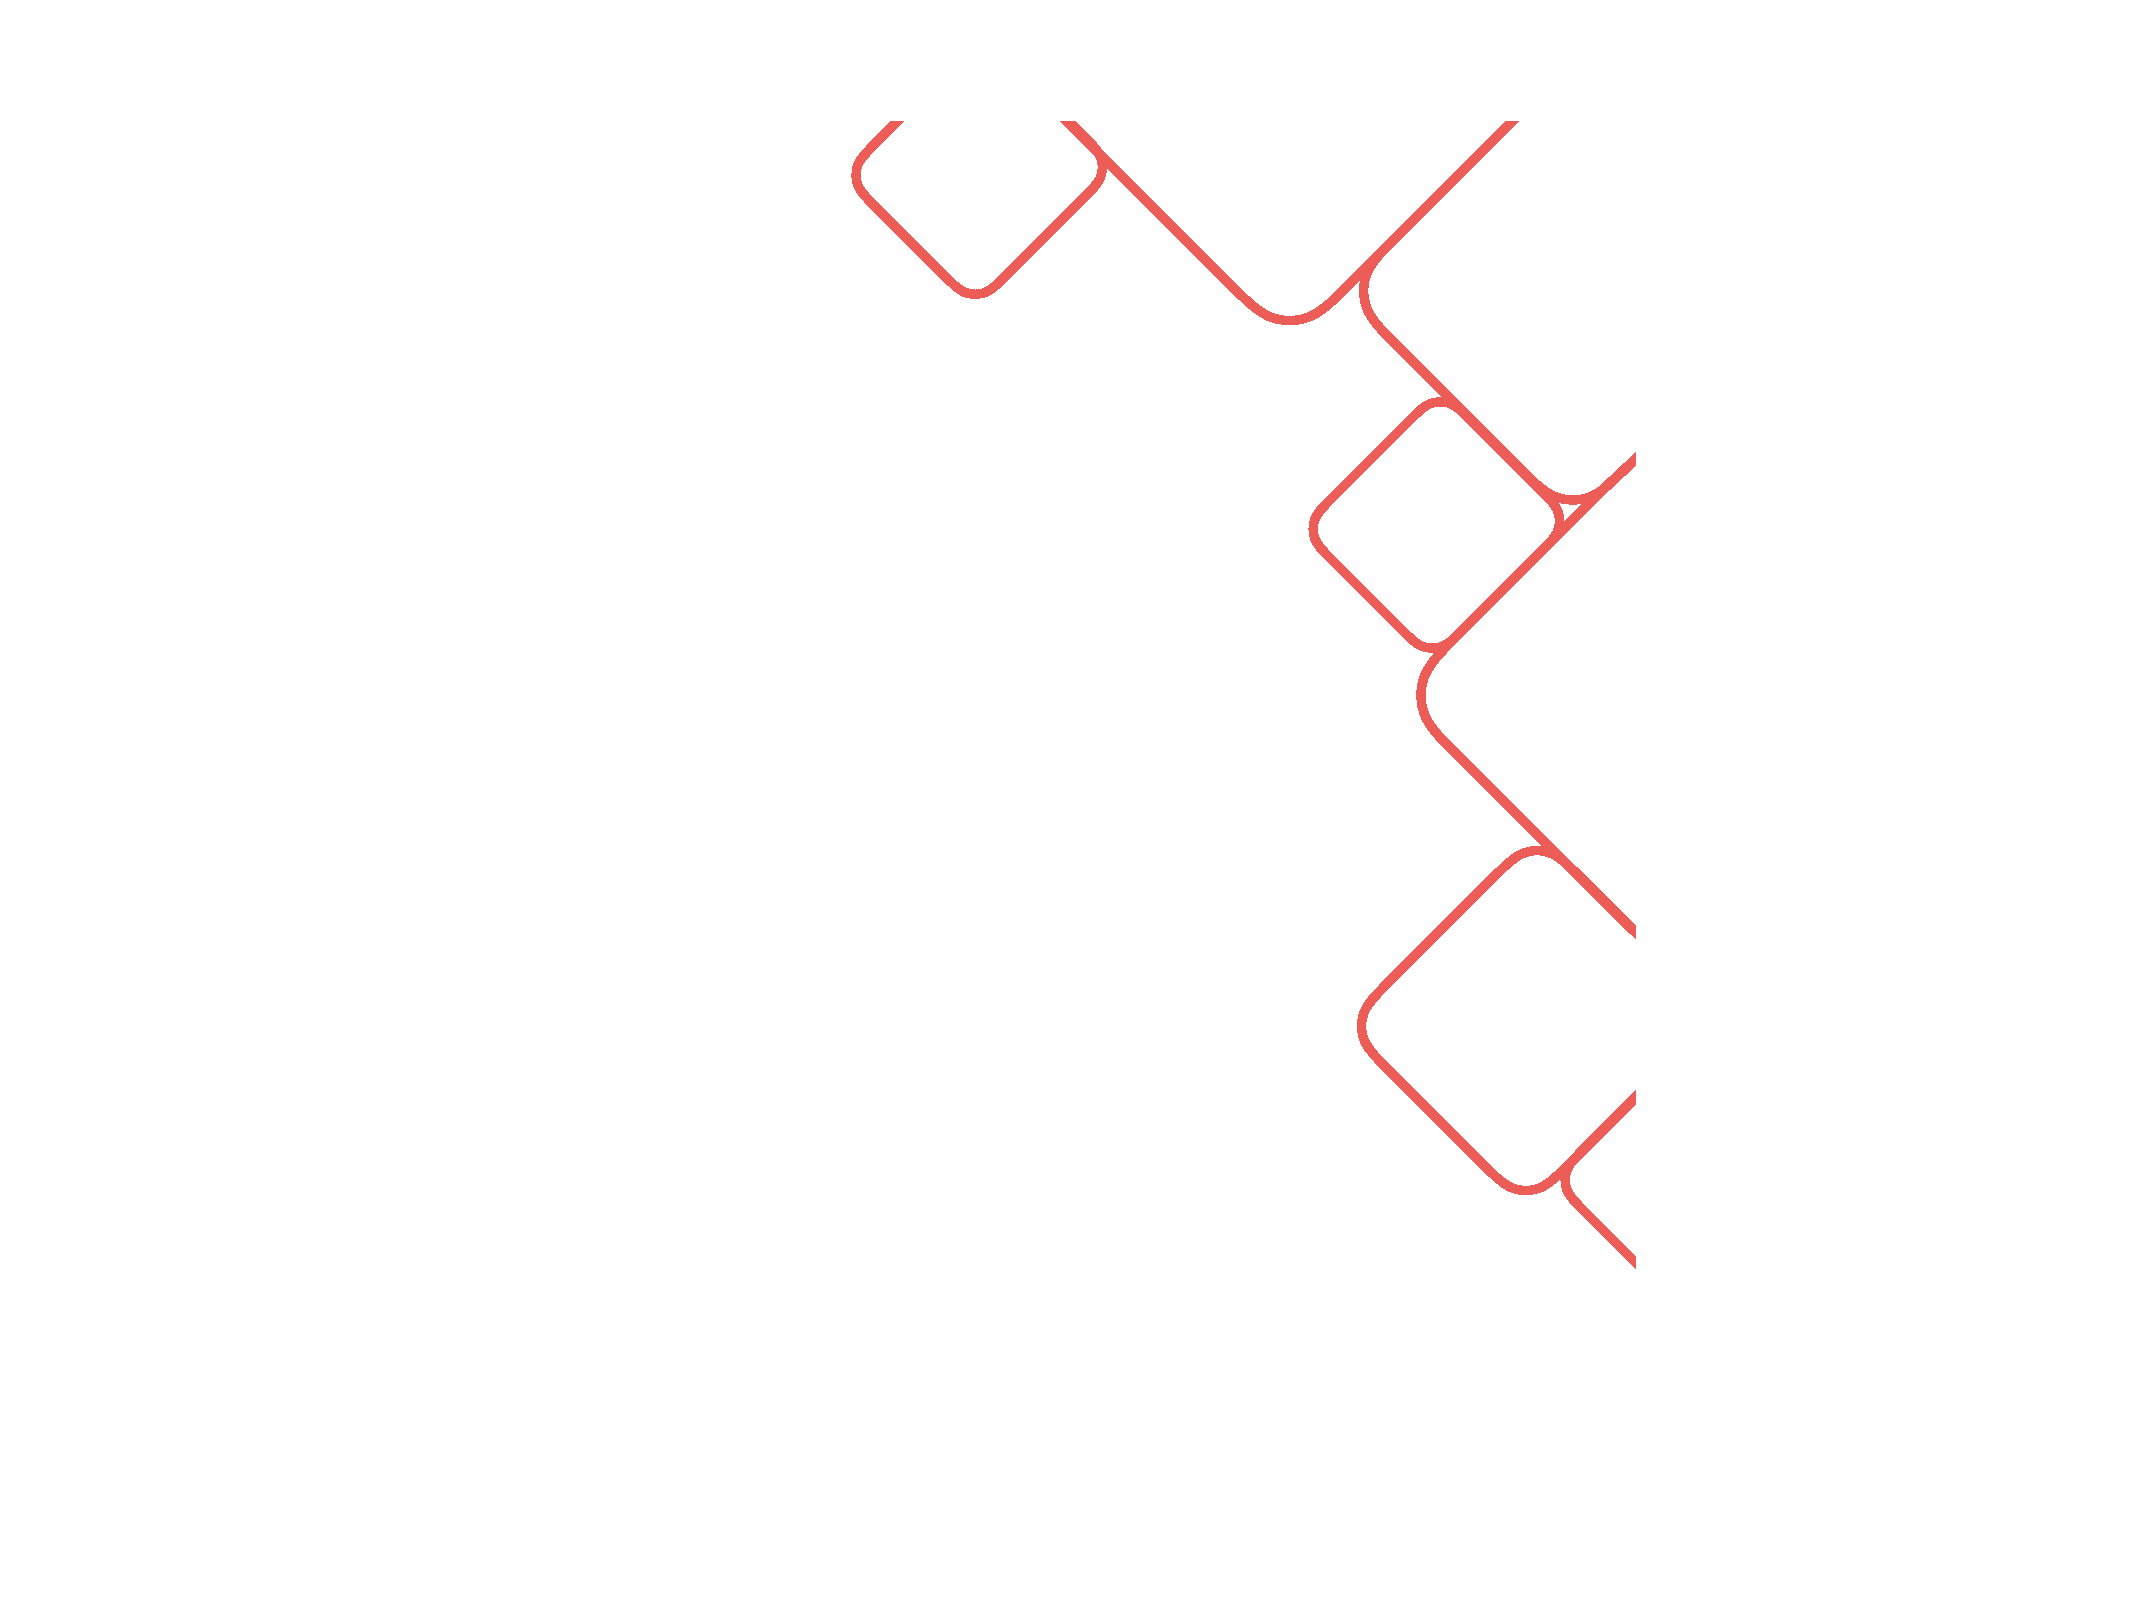
\includegraphics[width = \paperwidth,
   height = \paperheight, keepaspectratio]
   {cover.pdf}}}

% set option for code listing
%\lstset{language=IDL}
\lstset{basicstyle=\ttfamily}

% define the font for file names
\newenvironment{filenamefont}{\fontfamily{pcr}\selectfont}{\par}
\DeclareTextFontCommand{\filename}{\filenamefont}

% define the font for settings and structures ("pieces of code")
\newenvironment{codefont}{\fontfamily{cmtt}\selectfont}{\par}
\DeclareTextFontCommand{\code}{\codefont}


% Title page -------------------------------------------------------------------
% code taken from https://tex.stackexchange.com/questions/85904

\DeclareFixedFont{\titlefont}{T1}{ppl}{b}{}{0.5in}

\makeatletter
\def\printauthor{%
    {\Large \@author}}
\makeatother
\author{%
\textsc{Sirio Belli}
\texttt{sirio@mpe.mpg.de}
    }

\begin{document}

\begin{titlepage}

\vspace*{1cm}
\noindent
\Huge \textbf{\textit{Flame} user manual}\par
\vspace*{1cm}
\noindent
\Large Last updated \today \\
\null\vfill
\vspace*{1cm}
\noindent
%\hfill
\begin{minipage}{0.02\linewidth}
    \rule{1pt}{50pt}
\end{minipage}
\begin{minipage}{0.35\linewidth}
    \begin{flushleft}
        \printauthor
    \end{flushleft}
\end{minipage}
%

\end{titlepage}

% end title page -------------------------------------------------------------------

\newpage
\tableofcontents

\begin{sloppypar}

% ***********************************************************************************************
% ***********************************************************************************************
%									1. INTRODUCTION
% ***********************************************************************************************
% ***********************************************************************************************

\newpage
\section{Introduction}
\label{sec:introduction}

\flame\ is a pipeline for reducing near-infrared and optical multi-object spectroscopic data, written in IDL. The pipeline design and the algorithms used are described in Belli, Contursi \& Davies (2018, arXiv:1710.05924); users should read that paper before reading the present manual.

Although created specifically for the LUCI instrument at the Large Binocular Telescope, \flame\ has been designed in a modular way and can be easily adapted to work with the data produced by different instruments. For simplicity, the present document describes in detail the reduction of LUCI data. Section \ref{sec:instruments} explains how to use \flame\ with other supported instruments, and how it is possible to implement support for new instruments. There is also a minimal version of \flame\ (see Section \ref{sec:minimal}) that can be used to run simple diagnostics on data from virtually any instrument, which is particularly useful while observing.

If you made use of \flame\ in your work, please cite Belli, Contursi \& Davies (2018). For comments, bug reports, or suggestions please contact \texttt{sirio@mpe.mpg.de}, or post a message on the GitHub page.


% ***********************************************************************************************
% ***********************************************************************************************
%									2. INSTALLATION
% ***********************************************************************************************
% ***********************************************************************************************

%%%
%%% Note: the links do not show up on the pdf, even though they work if you know where to click.
%%%

\section{Installation}
\label{sec:installation}


\subsection{Requirements}

The pipeline has been extensively tested in Linux and Mac. Limited testing was done in Windows.

The following three external IDL libraries must be installed before running \flame:
\begin{enumerate}
\item NASA's IDL Astronomy User's Library\footnote{\url{http://idlastro.gsfc.nasa.gov/}};
\item David Fanning's Coyote Library\footnote{\url{http://www.idlcoyote.com/code_tips/installcoyote.php}};
\item Craig Markwardt's mpfit\footnote{\url{https://www.physics.wisc.edu/~craigm/idl/fitting.html}} (only the mpfit.pro and mpfit2dfun.pro files are needed).
\end{enumerate}
Make sure to have the most recent versions of these libraries (at least more recent than the January 2016 release).

Other third-party routines used by \flame\ are included in the distribution, in the \filename{flame/lib/} directory. These are the B-spline routines from the \texttt{idlutils} library, the L.A.Cosmic routine written by Joshua Bloom and Pieter van Dokkum, and the readmhdufits routine written by Marc Kassis.


\subsection{Download}

Download \flame\ from \url{http://siriobelli.github.io/flame/}. The parent directory \filename{flame/} contains the IDL code, documentation, and data needed to run the pipeline. You can either save this in the directory where you keep your IDL code, or save it somewhere else and then add the \filename{flame/} directory to the IDL path. No other step is necessary.





% ***********************************************************************************************
% ***********************************************************************************************
%									3. SETUP
% ***********************************************************************************************
% ***********************************************************************************************



\section{Setting Up the Data Reduction}
\label{sec:setup}


\subsection{Basic input}

Create a new, empty directory that will be used for the reduction of a data set. Then:
\begin{itemize}
\item Copy to this directory the appropriate driver file (for LUCI observations this would be \filename{flame\_driver\_luci.pro}) from the \filename{flame/drivers/} directory.
\item Create a text file (e.g., \filename{science.txt}) with, in each line, the full name, including the absolute path, of a raw science frame (either FITS files or gzipped FITS files).
\item \emph{(optional)} Create additional text files containing the names of the calibration frames (e.g., \filename{darks.txt}, \filename{flats.txt}, etc.)
\end{itemize}

The data reduction is controlled entirely via the driver file. Open the local copy with a text editor and have a look at the code. First the input parameters are set, the pipeline is then initialized, and finally the actual data reduction is run.

The first step in the driver file creates the \inp\ structure:
\begin{lstlisting}
 input = flame_create_input()
\end{lstlisting}
and the following steps populate the fields in the input structure. The data reduction is set up by modifying a few lines of code in the driver file.

\subsubsection{Science frames}
We start by specifying the name of the file containing the science frames; for example:
\begin{lstlisting}
input.science_filelist = 'science.txt'
\end{lstlisting}
If the file is not in the current working directory, then the absolute path must be provided.

\subsubsection{Nodding}
Near-infrared observations typically use spatial nodding for an effective sky subtraction. \flame\ supports a two-point nodding, also called A-B nodding, which is activated via the flag:
\begin{lstlisting}
input.AB_subtraction = 1
\end{lstlisting}

\subsubsection{Reference star}
It is always recommended to place a slit on a relatively bright star (hereafter called the reference star) from which the observing conditions and the spatial nodding can be accurately measured. In the A-B nodding scheme, the star trace will appear on two different positions, which may be in the same slit or in two different slits. The y pixel position of the reference star in both the A and the B position must be provided:
\begin{lstlisting}
input.star_y_A = 520
input.star_y_B = 560
\end{lstlisting}
These coordinates do not need to be exact. If the trace of the reference star is very faint in a single frame, a simple A-B subtraction is generally sufficient for a visual detection. When no reference star is available, the nodding pattern, if present, must be specified manually (see Section \ref{sec:manual_dithering}). If no AB nodding is performed, the B star position should be set to zero.

\subsubsection{Slits to be reduced}
While the default behavior is to reduce all the slits in the mask, it is sometimes preferable to reduce only one slit, for example to obtain a fast reduction for one representative object while observing. This can be achieved by specifying:
\begin{lstlisting}
input.reduce_only_oneslit = 2
\end{lstlisting}
where in this case we would get the reduction of only the second slit. The default value is zero which means that all slits will be reduced.

\subsubsection{Longslit observations}
Finally, to reduce longslit observations, it is sufficient to set the longslit flag:
\begin{lstlisting}
input.longslit = 1
\end{lstlisting}
Since the longslit typically spans the whole detector in the vertical range, the edges of the longslit are not well defined. The region of interest must be specified by providing the y pixel coordinates of the top and bottom limits:
\begin{lstlisting}
input.longslit_edge = [1050, 1350]
\end{lstlisting}
If \code{longslit\_edge} is set to [0,0], the default is to reduce the full frame excluding 10\% of pixels at the bottom and 10\% at the top. For example, for a frame that is 2048 pixels tall, this would correspond to the [205, 1843] range.


\subsection{Optional input}

The \inp\ structure contains additional fields that can be used to specify optional inputs. The full list is reported in Table \ref{tab:input}, and the content of the \inp\ structure can be explored at any time by typing
\begin{lstlisting}
help, input
\end{lstlisting}
in the interactive IDL session.

% ******************************************************************************
\begin{table}
\caption{Content of the \inp\ structure \label{tab:input}}
\medskip
\footnotesize
\makebox[\textwidth][c]{
  \begin{tabular}{lll}
    \hline
    \smallskip
    Field    & Default Value   & Description \\
    \hline
    \smallskip
science\_filelist   	     & 'science.txt' 		& name of ASCII file containing the list of science frames \\
AB\_subtraction      & 0      & flag to enable AB subtraction \\
star\_y\_A 		 & 0			& pixel y-coordinate of the A position of the star trace \\
star\_y\_B 		 & 0			& pixel y-coordinate of the B position of the star trace \\
reduce\_only\_oneslit 	& 0 				& if equal to $n$ and non-zero, reduce only the $n$-th slit \\
longslit 				& 0 				& set to $1$ to reduce long-slit data \\
longslit\_edge			& [0, 0] 			& when reducing long-slit data, only consider this range of pixel y-coordinate \\
dark\_filelist   		       & 'none' 				& name of ASCII file containing the list of dark frames\\
pixelflat\_filelist        & 'none' 				& name of ASCII file containing the list of frames for pixel flat field	\\
illumflat\_filelist   		 & 'none' 				& name of ASCII file containing the list of frames for illumination flat field	\\
illumflat\_pixelshift  		 & 0      				& vertical pixel shift required to align the illumination flat with the science frames	\\
slitflat\_filelist    & 'none'        & name of ASCII file containing the list of slit flats \\
slitflat\_pixelshift  & 0      				& vertical pixel shift required to align the slit flat with the science frames	\\
arc\_filelist   		  & 'none' 				& name of ASCII file containing the list of lamp arc frames	\\
arc\_pixelshift  		  & 0      				& vertical pixel shift required to align the arc with the science frames	\\
slit\_position\_file  & 'none'        & name of ASCII file containing the approximate y-coordinates of the slit edges \\
dither\_file       		& 'none' 				& name of ASCII file containing the list of dither positions \\
max\_slitwidth\_arcsec & 0          & threshold value of the slit width used to identify the alignment boxes \\
intermediate\_dir		 & 'intermediate/'		& directory that will contain the intermediate products \\
output\_dir				   & 'output/'			& directory that will contain the final output \\
\hline
\end{tabular}
}
\end{table}
% ******************************************************************************


\subsubsection{Calibration frames}
The calibration frames used by \flame\ are the dark frames, pixel flats, illumination flats, slit flats, and arcs. Each of these types of calibrations can be supplied to the pipeline via text files containing a list of FITS files, similarly to what done for the science data. The only difference is that all the calibration files are optional, and the default value for the filelist parameter is always \texttt{'none'}. Here is an example:
\begin{lstlisting}
input.dark_filelist = 'darks.txt'
input.pixelflat_filelist = 'pixelflats.txt'
input.illumflat_filelist = 'none'
input.slitflat_filelist = 'twilightflats.txt'
input.arc_filelist = 'none'
\end{lstlisting}
For the illumination flats, slit flats, and arcs, it is important that the calibration frames are spatially aligned with the science frames. However, it is often the case that calibrations taken in the afternoon show a vertical displacement compared to science observations because of flexure. In this case, it is possible to correct for this by specifying the vertical offset, in pixel, that must be applied to the calibration frames:
\begin{lstlisting}
input.illumflat_pixelshift = 7
input.slitflat_pixelshift = 8
input.arc_pixelshift = 0
\end{lstlisting}

\textbf{Warning:} the use of arcs with LUCI observations has not been tested.


\subsubsection{Slit edge positions}
Normally, the expected positions of the slits on the detector are derived from the values in the FITS header. However, sometimes this can fail, particularly when the slits are tilted or curved. In these cases it is possible to specify the list of approximate pixel positions of each slit edge as an ASCII file:
\begin{lstlisting}
input.slit_position_file = 'slit_edges.reg'
\end{lstlisting}
The easiest way to generate this file is to open the slit flat field (or a science frame) with ds9, make a simple circular region at each slit edge (both top and bottom edges for each slit must be specified), and save the regions in a file with format 'XY' and coordinate system 'Image'.


\subsubsection{Dithering positions}
\label{sec:manual_dithering}
It is advisable to always have a reference star on the multi-slit mask. When this is not possible, \flame\ cannot measure the nodding and dithering offset for each frame, and this pattern needs to be saved in an ASCII file. The file must contain a number of lines equal to the number of science frames. Each line will have the value of the vertical offset, \textbf{in pixels} (note that earlier versions of \flame\ required the input in arcseconds instead), corresponding to that frame; for example 25, -25, 25, -25, etc. Then the file name needs to be input in the \inp\ structure:
\begin{lstlisting}
input.dither_file = 'dither.txt'
\end{lstlisting}


\subsubsection{Alignment Box Identification}
Each slitmask has typically a few wide slits which are used for alignment. \flame\ ranks the slits by their width, and discards all those with the largest width, assuming those are the alignment boxes. However, it is possible that the alignment boxes have different width, in this case the user needs to specify a threshold so that the alignment boxes can be identified and discarded. For example, if all science slits in a mask are narrower than $2"$, one can specify:
\begin{lstlisting}
input.max_slitwidth_arcsec = 2.0
\end{lstlisting}


\subsubsection{Directories}
Finally, it is possible to specify the directories for intermediate and final outputs:
\begin{lstlisting}
input.intermediate_dir = 'intermediate/'
input.output_dir = 'output/'
\end{lstlisting}
If these directories do not exist, they will be created by \flame. Note that these definitions use relative paths, but absolute paths can also be used.



\subsection{Initialization}

The data reduction in \flame\ consists of a series of steps, which are represented by individual routines. The information is carried from one routine to the next via a structure, named \fuel, which contains all the input parameters set by the user, together with all the internal variables.

Once the \inp\ fields have been specified, the \fuel\ structure must be created:
\begin{lstlisting}
fuel = flame_initialize_luci(input)
\end{lstlisting}
This will also check for potential errors in the inputs, and create the necessary directories.

The \fuel\ structure consists of six substructures:
\begin{itemize}
	\item fuel.input: a copy of the \inp\ structure created in the previous step;
  \item fuel.settings: a series of settings and parameters that control the data reduction;
	\item fuel.util: utility variables needed by \flame;
	\item fuel.instrument: instrument-specific information;
	\item fuel.diagnostics: diagnostics such as seeing and transparency for each of the science frames;
	\item fuel.slits: information relative to each slit, such as position on the detector and expected wavelength range.
\end{itemize}

Some of the fields in the \fuel\ structure are initially set to null pointers and will be created by successive steps.

During the initialization, relevant fields from the FITS header of the science files, such as band, central wavelength, and slit positions are read and saved. This is the only step during the data reduction where instrument-specific operations are performed.

After the initialization, the user has complete control over the \texttt{fuel.settings} structure. We will describe some of the settings in the next section; the complete list together with a brief description for each of them is shown in Table \ref{tab:settings}. Normally, the user should not edit the other five substructures contained in \fuel.

% ******************************************************************************
\begin{table}
\caption{Content of the \texttt{fuel.settings} structure \label{tab:settings}}
\medskip
\footnotesize
  \makebox[\textwidth][c]{
  \begin{tabular}{llll}
    \hline
    Field    & Default Value   & Routine   & Description \\
             & (for LUCI)      &           & \\
    \hline
    \smallskip
    sky\_emission\_filename       &               & (many)           & file with model spectrum of sky emission \\
    linelist\_sky\_filename       &               & (many)           & file with list of sky emission lines \\
    linelist\_arcs\_filename      &               & (many)           & file with list of arcs emission lines \\
    star\_x\_range 			          & [1000, 1200]  & diagnostics   	 & range of pixel x-coordinate to consider for the reference star trace \\
    star\_y\_window               & $\simeq$4 arcsec & diagnostics   & range of pixel y-coordinate to consider for the reference star trace \\
    clean\_individual\_frames     & 0             & calibrations     & identify and mask cosmic rays in each frame \\
    badpix\_useflat               & 1             & calibrations     & use pixel flat field (if provided) to identify bad pixels \\
    badpix\_usedark               & 1             & calibrations     & use dark frames (if provided) to identify bad pixels \\
    badpix\_sigma                 & 7.0           & calibrations     & sigma clipping to identify bad pixels in the master dark frame \\
    badpix\_flatcorrection        & 0.20          & calibrations     & values beyond this deviation in the master pixel flat are bad pixels \\
    flatfield\_data               & 1             & calibrations     & divide the science data by the master pixel flat field (if provided) \\
    darksub\_data                 & 0             & calibrations     & subtract the master dark (if provided) from the science data \\
    trace\_slit\_with\_emlines    & 1             & slitid           & use emission lines (e.g., from sky or arcs) to trace slit edges \\
    trace\_slit\_xmargin          & 20            & slitid           & horizontal margin (in pixels) to consider around each emission line \\
    trace\_slit\_ymargin          & 12            & slitid           & vertical margin (in pixels) to consider beyond the expected slit edge \\
    trace\_slit\_polydegree       & 2             & slitid           & degree of the polynomial used to describe the slit edge \\
    trace\_longslit               & 0             & slitid           & approximate vertical position of a bright trace (used for the rectification) \\
    trim\_slit                    & [0, 0]        & cutouts          & limits, in x pixel coordinates, used to trim the cutouts \\
    spatial\_resampling           & 1.0           & spatialcal       & resampling factor for the spatial direction \\
    roughwavecal\_R               & [500, 1000, 3000] & roughwavecal & spectral resolution to be used for the rough wavelength calibration \\
    roughwavecal\_smooth\_window  & 20            & roughwavecal     & window, in pixels, used to calculate and subtract the sky continuum \\
    roughwavecal\_split           & 0             & roughwavecal     & in the last step of rough\_wavecal, split the wavelength range in two \\
    findlines\_stack\_rows        & 0             & findlines        & number of pixel rows to stack when identifying arcs or sky lines \\
    findlines\_poly\_degree       & 5             & findlines        & polynomial degree for the row-by-row wavelength solution \\
    findlines\_Nmin\_lines        & 6             & findlines        & number of lines below which a pixel row is discarded \\
    findlines\_linefit\_window    & 6.0           & findlines        & window used for Gaussian fitting, in units of expected line width \\
    wavesolution\_order\_x        & 3             & wavecal          & polynomial degree for the wavelength solution, along x \\
    wavesolution\_order\_y        & 2             & wavecal          & polynomial degree for the wavelength solution, along y \\
    wavecal\_sigmaclip            & 3.0           & wavecal          & rejection threshold when fitting the 2D wavelength solution \\
    shift\_arcs                   & 1             & wavecal          & apply wavelength shift calculated from sky lines to the arcs solution \\
    shift\_arcs\_Nmin\_lines      & 1             & wavecal          & minimum number of sky lines needed for shifting the arcs solution \\
    illumination\_correction      & 1             & illumcorr        & apply illumination correction to science frames \\
    skysub                        & 1             & skysub           & construct and subtract a model of the sky \\
    skysub\_plot                  & 0             & skysub           & while fitting the sky, show pop-up windows with the B-spline fit \\
    skysub\_plot\_range           & [0.4, 0.6]    & skysub           & fractional range of the x axis to plot during sky subtraction \\
    skysub\_bspline\_oversample   & 1.0           & skysub           & breakpoints separation for the B-spline model, in units of pixels \\
    skysub\_reject\_fraction      & 0.10          & skysub           & fraction of pixels to reject at each loop \\
    skysub\_reject\_loops         & 3             & skysub           & number of loops for outlier rejection \\
    skysub\_reject\_window        & 2.0           & skysub           & window for outlier rejection, in units of breakpoint separation \\
    interpolation\_method         & 'NaturalNeighbor'  & rectify     & method used to resample frames during rectification \\
    frame\_weights                & 'None'        & combine          & weights to use for the final frame stacking \\
    combine\_sigma\_clip          & 2.0           & combine          & sigma-clipping to use when combining frames \\
    combine\_min\_framefrac       & 0.49          & combine          & minimum fraction of frames that must contribute to a pixel \\
    extract\_optimal              & 1             & extract          & use optimal extraction instead of boxcar extraction \\
    extract\_gaussian\_profile    & 1             & extract          & use Gaussian fit to determine weights for optimal extraction \\
    stop\_on\_error               & 1             & (all)            & halt execution when an error occurs \\
    \hline
  \end{tabular}
  }
\end{table}
% ******************************************************************************




% ***********************************************************************************************
% ***********************************************************************************************
%									4. DATA REDUCTION
% ***********************************************************************************************
% ***********************************************************************************************



\section{Running the Data Reduction}
\label{sec:data_reduction}

Once the first part of the driver file has been edited, the data reduction can be executed. Broadly speaking there are two ways to run \flame:
\begin{enumerate}
\item The user can copy line-by-line the content of the driver file into an interactive IDL session. This allows the user to check the result of each individual step, exploring the \fuel\ structure and the output files and plots.

\item The driver can be executed automatically, by typing:
\begin{lstlisting}
.run flame_driver_luci.pro
\end{lstlisting}
in the IDL command line (assuming the driver file is located in the current directory). The \code{.run} command executes a file as an IDL \emph{main program}, which means that the driver file must have an END statement but does not need a PRO statement at the beginning, as opposed to regular routines\footnote{Technically, the driver file can also be executed as a \emph{batch file}, by running \code{idl flame\_driver\_luci.pro} at the UNIX command line, although this will produce an error message when the END statement is encountered. This method is discouraged because if one of the modules produces an error, the execution will not stop but will continue with the remaining modules, making it difficult for the user to understand the source of the problem.}.
\end{enumerate}

The driver file contains fifteen steps or modules. Every module is an IDL routine whose name starts with \code{flame\_} and which is saved in a .pro file with the same name in the directory \filename{flame/pro/}. All modules accept (and require) only one argument, which is the \fuel\ structure, so that the IDL code for each module looks the same:
\begin{lstlisting}
flame_modulename, fuel
\end{lstlisting}

Every module edits the fuel structure and/or outputs files in the intermediate directory. Only the last three modules, which create the final results, save the output files in the output directory. Furthermore, at the end of each module the \fuel\ structure is saved as an IDL save file in the intermediate directory, so that the execution can be interrupted and restarted, even in a new IDL session, as long as the \fuel\ structure is loaded with
\begin{lstlisting}
restore, 'intermediate/fuel.sav'
\end{lstlisting}

In this section we describe the goal, output products, and potential issues for each step in the data reduction. For each module we also discuss the available settings; however it is preferable to set all the options before starting the data reduction, i.e., immediately after the initialization.

\medskip
\noindent
\textbf{Note:} All wavelengths used in \flame\ are measured in vacuum and in units of micron, except for the 1D extracted spectra which are in units of angstrom to preserve compatibility with third-party software.




% ---------------------------------------------------
\subsection{\texttt{flame\_diagnostics}}
\label{sec:diagnostics}

The first step produces important diagnostics which will be used by other modules. These diagnostics can also be helpful to the user to assess the quality of the observations, and can be run in real time while observing, ideally after every new frame or frame pair has been taken.

\begin{figure}[htbp]
\centering
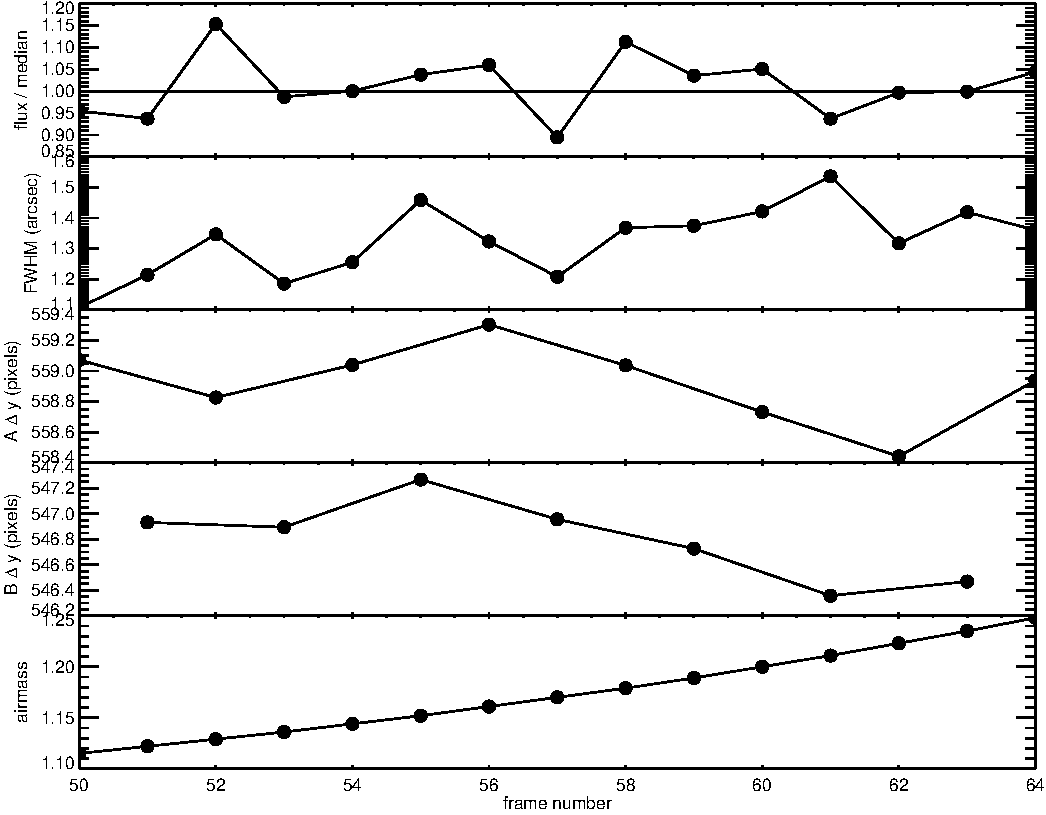
\includegraphics[width=0.9\textwidth]{diagnostics}
\caption{Example of diagnostic plots. From the top: Flux of the star trace, normalized by the median value; FWHM in arcsec; vertical position of the trace in the A frames; vertical position of the trace in the B frames; airmass value read from the FITS header.}
\label{fig:diagnostics}
\end{figure}

Starting with the y coordinates specified by the user in the \inp\ structure, this module detects the reference star position on each frame, and identifies which frames belong to the $A$ and which to the $B$ position (and assigns an $X$ position when no star trace is found). Then, for each frame a Gaussian profile is fit to the star trace, from which the flux, vertical position and FWHM are measured. In addition, the airmass value is read from the FITS header of each frame.

All these quantities are saved in the substructure \code{fuel.diagnostics} and plotted as a function of the frame number in the file \filename{diagnostics.ps}. One example of such file is shown in Figure \ref{fig:diagnostics}. Because of nodding, the vertical position is shown in different panels for the $A$ and the $B$ frames.

The diagnostic plots can be used to judge the trend of transmission (including the effect of cloud cover), seeing, and drift. In addition to help the user make informed decisions while observing, these measurements are also useful to identify the bad frames that should be excluded from the final data reduction.

\medskip
\noindent
\textbf{Outputs.} The main output file is \filename{diagnostics.ps}; the same information is also available in tabular form in \filename{diagnostics.txt} (these two files are also saved to the output directory, for reasons explained in Section \ref{sec:final_output}).  It is a good idea to check that each frame has been assigned to the correct nodding position, and that the measured seeing, flux variation, and position are reasonable. If one or more frames have unexpected values, additional plots written to \filename{startrace\_identify\_AB.ps} and \filename{startraces.ps} should be checked.

\medskip
\noindent
\textbf{Troubleshooting.} If some of the fits to the stellar trace fail, there are three things that the user can do:
\begin{enumerate}
\item The input values (\code{input.star\_y\_A} and \code{input.star\_y\_B}) can be slightly adjusted. Particularly if the first frame was used as a reference, and there is substantial drift among frames, choosing a value that is more representative of all frames can help. When the trace is tilted with respect to the detector rows, it should be checked that the vertical position of the trace is measured at the correct x position (see next point).
\item The stellar trace is extracted from a relatively narrow range of $x$ pixels, which can be changed via \texttt{settings.star\_x\_range}. Sometimes the stellar spectrum only covers part of the detector, for example if the slit was placed at the left or right edge of the mask. If sky lines are strong, it is advisable to choose a relatively clear, narrow range; if the star is very faint, it may be better to use a wider range.
\item The vertical window used to extract the stellar profile can also be changed, via \texttt{settings.star\_y\_window}. The stellar trace should be within this window in all frames, so a wider window should be used when dealing with large drift or dithering. Sometimes fits can fail because the spatial profile is disturbed by the presence of the slit edge; in these cases the size of the window should be decreased.
\end{enumerate}


% ---------------------------------------------------
\subsection{\texttt{flame\_quickstack}}
\label{sec:quickstack}

The second step produces a FITS file which is the stack of the A frames or, in the case of $A-B$ nodding, the difference of a stack of the $A$ frames and a stack of the $B$ frames. This step is also useful while observing, since the simple $A-B$ subtraction often yields a decent sky removal which allows the detection of faint continuum traces or emission lines.

The sole goal of this module is to allow a quick look at the data. This step can be skipped with no consequences for the remaining parts of the data reduction.

This step and the previous ones can be run on virtually any data set without any knowledge on the instrument except for the spatial pixel scale. This minimal version of \flame, designed for on-the-fly use, is described in Section \ref{sec:minimal}.

\medskip
\noindent
\textbf{Outputs.} The only output is the file named \filename{quickstack\_A-B.fits} or similar (according to the nodding pattern).


% ---------------------------------------------------
\subsection{\texttt{flame\_calibrations}}
\label{sec:calibrations}

This module applies a number of calibrations to the raw science frames. First, the bad pixel mask is generated from the input dark and/or flat frames. If neither dark nor flat field frames were supplied, then the default bad pixel mask, stored in \filename{flame/data/}, is used. The flat field correction and dark subtraction are then performed.

In order to offer the maximum flexibility, individual corrections can be turned on or off \emph{even when the corresponding frames have been supplied to \flame}. For example, if the pixel flat field frames are provided, the user can choose whether they should be used for the flat field correction with the \code{settings.flatfield\_data} option, and whether they should be used for the bad pixel identification via the \code{settings.badpix\_useflat} option. Analogous settings apply to the dark frames.

When using the flat field to construct the bad pixel mask, the option \code{settings.badpix\_flatcorrection} controls the threshold used to identify bad pixels. A similar option (\code{settings.badpix\_sigma}) exists for when the darks are used. If darks and flats are not used then the default bad pixel mask will be used. Users that wish to skip the bad pixel flagging altogether need to additionally set \code{fuel.instrument.default\_badpixel\_mask = 'none'}

It is also possible to clean individual frames of cosmic rays using L.A.Cosmic, but this is generally not needed for LUCI data, as long as the number of frames is enough for an effective sigma-clipping.

\medskip
\noindent
\textbf{Outputs.} After all the calibrations have been applied, the `corrected' science frames are saved in the \filename{intermediate/frames/} directory. Each FITS file contains a second extension with the error spectrum, which is calculated as the combination of read-out noise and Poisson noise; both extensions are in units of electron per second. The \code{master\_slitflat.fits} file is also saved in the intermediate directory. Additional files may be saved, depending on the options used. These include the master flats and darks, the median pixel flat (which is a simple median stack, not normalized, and is used to obtain the master file), the bad pixel mask, and ps files showing the distribution of pixel values in the master flats and/or darks and the threshold used to identify bad pixels. If present, the master pixel flat and bad pixel mask should be checked to make sure they look reasonable.


\medskip
\noindent
\textbf{Note.} The flat field frames are never dark-subtracted. For a proper dark-subtraction, an additional set of dark frames matching the exposure time of the flat field (which is generally different from the exposure time of the science frames) is needed. In order to have a simple and user-friendly pipeline, \flame\ does not perform this extra step; however users can easily dark-subtract each flat field frame before feeding them to \flame. This is generally not needed because most modern detectors have a low dark current, and as long as the counts in the flat fields are high, this correction is negligible.

In order to allow users to pre-process the calibration frames, the counts in the flat field are normalized and the uncertainty on the observed flux is not calculated nor propagated to the reduced data. Users need to make sure that the counts in the flat field frames are high enough so that the Poisson error in the master flat is negligible compared to the uncertainty in the science data.


\begin{figure}[htbp]
\centering
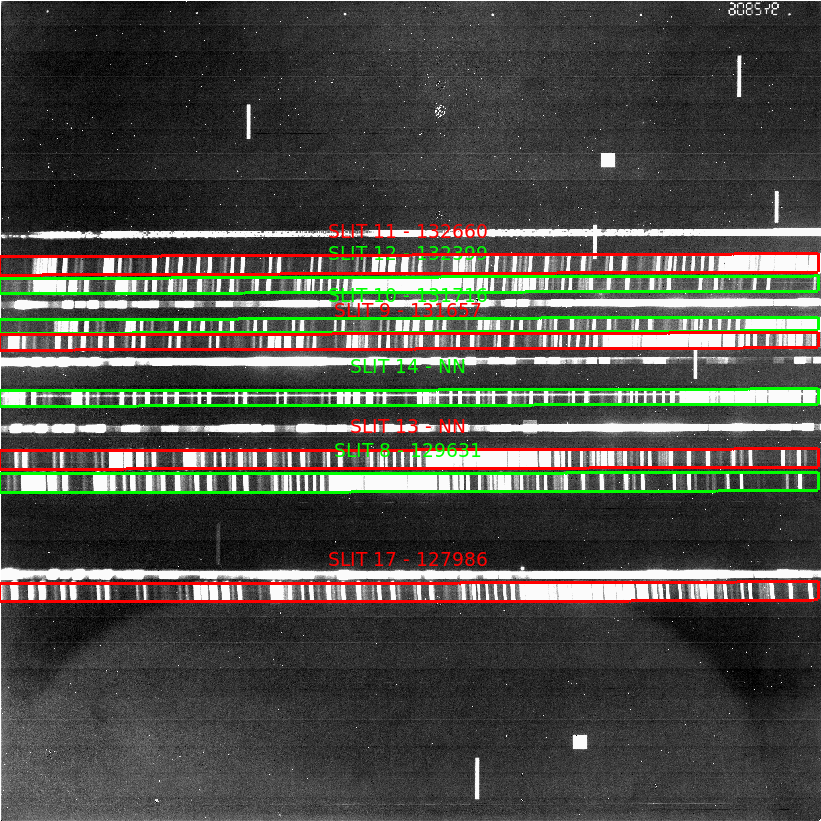
\includegraphics[width=0.9\textwidth]{slits}
\caption{An example of LUCI raw frame, with the regions marking the slits identified by \flame\ shown in red and green. The slits that are not marked are the boxes for the alignment stars, which are ignored by the pipeline.}
\label{fig:slits}
\end{figure}

% ---------------------------------------------------
\subsection{\texttt{flame\_slitid}}
\label{sec:slitid}

The module \texttt{flame\_slitid} is responsible for identifying the slits in the master slit flat. The vertical coordinates of the slit edges calculated during the initialization are used. However, the physical position of the mask with respect to the detector is typically difficult to predict and varies slightly from one night to the other. To account for this, a vertical shift is calculated by identifying the approximate slit positions.

Once the approximate pixel position of each slit has been calculated, a second, more refined slit edge detection is run. This is based on the identification of individual OH emission lines, which are typically very bright and can be reliably used to trace the edge of a slit. For each slit, a low-order polynomial is fit to the $y$ coordinate of the edge as a function of $x$ position, and the results are saved to the fuel structure. The order of the polynomial can be specified via the settings.

In some cases, particularly in the $K$ band (and for optical instruments), there are not enough bright OH lines for identifying the slit edges. It is possible to use the continuum emission instead, by specifying \code{settings.trace\_slit\_with\_emlines=0}. Using lamp flats or arc frames as the slit flat field is also an option.

\medskip
\noindent
\textbf{Notes on long slit data.} When reducing a long slit, there are no slit edges that can be tracked, therefore the spectra are not spatially rectified. However, if a bright trace is present in the spectrum (either from the science target itself or from another object on the slit, possibly close to the science target), it can be used to calculate the spatial rectification. In this case, the approximate vertical coordinate of the trace (corresponding to x-positions in the center of the detector) must be specified, e.g. \code{settings.trace\_longslit=854}.

The trace needs to be clearly visible in the slit flat field, which is often not the case when using the default options. Usually, the best result is obtained when using the quickstack image as slit flat field. Here is how to achieve this: run the first two steps of \flame\ in order to produce a quickstack image; change the name of the quickstack file into, for example, \code{slitflat.fits}; make an ASCII file (e.g., \code{slitflat.txt}) with only one line, which is the name of the FITS file; specify the slit flat in the driver (e.g., \code{input.slitflat\_filelist = 'slitflat.txt'}); specify also the \code{settings.trace\_longslit} (keep in mind that the pixel coordinate of the trace must be measured in the slit flat field itself); finally run \flame\ from the beginning.

\medskip
\noindent
\textbf{Outputs.} This module creates the file \filename{slits.reg}, which is a ds9 region file that can be loaded on top of the slit flat (or any science frame) and will show the slit edges (see Figure \ref{fig:slits}). This can be used to check the slit detection and also to identify which slit on the science frame corresponds to which target. The raw detection (i.e., before the polynomial fit) of the slit edges are saved in \filename{slits\_raw.reg}.

\medskip
\noindent
\textbf{Troubleshooting.} If the slit identification fails or is not accurate, the user can change the vertical size of the cutout used for the slit identification. If emission lines are used, a cutout is produced around each line, and the horizontal dimension of the cutout can also be changed. In these cases the \filename{slits\_raw.reg} file is more helpful because it shows the individual detections, and can be used to guide the tweaking of the parameters.

In very difficult cases, an alternative approach is to use the longslit option to manually select the region within one slit to reduce. By default the longslit option assumes that the slit is \emph{spatially} centered on the mask. If this assumption causes a wildly wrong initial guess for the wavelength range, it is possible to override this value by changing the \texttt{fuel.slits.range\_lambda0} variable, which is a 2-element array containing the minimum and maximum values to be considered for the wavelength of the first pixel.


% ---------------------------------------------------
\subsection{\texttt{flame\_cutouts}}
\label{sec:cutouts}

Using the slit definition from the previous step, the slits are extracted from each corrected frame and saved as FITS files. Sometimes it may be useful to reduce only a subset of the observed spectrum, for example to speed up the reduction or to avoid a spectral region for which the wavelength calibration is challenging. In these cases it is possible to specify the range in x pixel coordinates to be considered via the \code{settings.trim\_slit} option (e.g., setting it to [0, 1023] would mean that only the left half of the LUCI detector will be reduced).

\medskip
\noindent
\textbf{Note:} From this step on, the outputs are saved in a subdirectory for each slit, e.g. \code{intermediate/slit07} for slit number 7.

\medskip
\noindent
\textbf{Outputs.} For each slit, a cutout is produced for each frame, and saved as a FITS file. Similarly to the corrected frames, the cutouts are in units or electrons per second and include a second extension with the error spectrum.


% ---------------------------------------------------
\subsection{\texttt{flame\_spatialcal}}
\label{sec:spatialcal}

The spatial rectification is calculated starting from the slit edges, and is corrected for nodding and dithering using the results of the diagnostics. The coefficients of the coordinate transformation $\gamma(x,y)$ are stored for each cutout in the \code{fuel.slits} structure. By default, the spatial side of the rectified pixels is identical to that of the raw, observed pixels: $\Delta \gamma = \Delta y$. However there are rare cases when a user may want to change this: for example when using the N3.75 camera with LUCI the two detectors end up having slightly different spatial scales. In this case it is best to change the spatial scale for the data from one or both eyes so that the output spectra can be easily combined without having to further interpolate the data. This can be done by changing the value of \code{settings.spatial\_resampling}.

\medskip
\noindent
No outputs are created during this step.


% ---------------------------------------------------
\subsection{\texttt{flame\_roughwavecal}}
\label{sec:roughwavecal}

The wavelength calibration is arguably the most important and difficult step in the data reduction. An accurate calibration is not only useful for the scientific interpretation of the data, but is also necessary for a correct sky subtraction.

In \flame, the wavelength calibration is split into three steps. The first step finds an approximate wavelength calibration for the central part of the slit, using only the first science frame. The sky spectrum is extracted from the central five pixels of the slit, and is compared to a model spectrum. The comparison consists of two successive steps:
\begin{enumerate}
\item Both the observed and the model sky spectra are smoothed to an intermediate spectral resolution ($R=500$, but this value can be controlled via settings.roughwavecal\_R), and a series of values for the pixel scale (in micron per pixel) are tested. At each loop, cross-correlation is used to find the initial wavelength, and the pixel scale that gives the largest value of the cross-correlation is selected.
\item Once the pixel scale and the initial wavelength are roughly known, a finer comparison is performed. In this case the spectra are not heavily smoothed, so that the narrow OH lines can be used for a very effective comparison. The relation between $x$ pixel coordinate and wavelength is typically not linear, and a second-order polynomial is used: $\lambda(x) = a_0 + a_1 x + a_2 x^2$. A fine grid of values for $a_1$ and $a_2$ is used, and at each loop cross-correlation is used to determine the best value for $a_0$.
\item Finally, another cross-correlation is performed at the native spectral resolution.
\end{enumerate}

\medskip
\noindent
\textbf{Outputs.} For each slit, plots illustrating the successive comparisons of observed and model sky spectra are saved as ps files (rough\_wavelength\_calibration.ps) in the slit directory. An example is shown in Figure \ref{fig:wavecal_approx}.

\medskip
\noindent
\textbf{Troubleshooting.} The spectral resolution $R$ used in the three steps is stored in \code{settings.roughwavecal\_R} and can be tweaked when the default values are not satisfactory. When the wavelength solution is highly non-linear, or the wavelength range is extended, it may be difficult to obtain an accurate fit using a second-order polynomial. In these cases the user can set \code{settings.roughwavecal\_split}, and the third step will be performed on the two halves of the spectrum separately, with a substantial increase in the flexibility of the wavelength solution.

If the sky spectrum includes a strong contribution from continuum emission, as is often the case for the thermal emission in the K band, it may be necessary to fit and subtract a low-order polynomial to the observed spectrum before comparing it to the model. This is controlled by the parameter \code{settings.roughwavecal\_smooth\_window}.

If arcs were provided, then the rough wavelength calibration will be performed using a model of the arcs spectrum instead of the sky spectrum. One important difference is that this arcs spectrum is not stored in a file, but is generated on the fly from the arcs line list. If this model spectrum does not look similar to the observed arcs, the user can adjust the arcs line list, as discussed in Section \ref{sec:wavecal}, and run again the rough wavelength calibration.


\begin{figure*}[tbp]
\begin{minipage}{\textwidth}
   \centering
 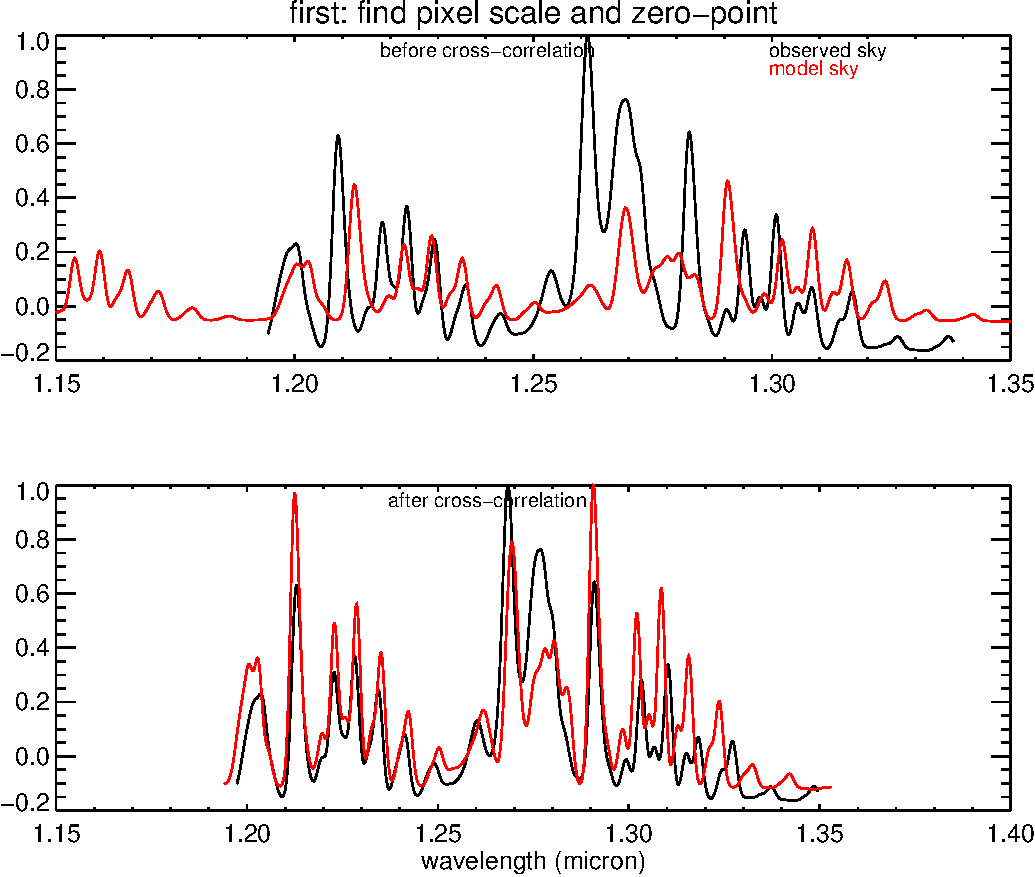
\includegraphics[width=0.31\textwidth]{wavecal1}
   \hspace*{0.01\textwidth}
 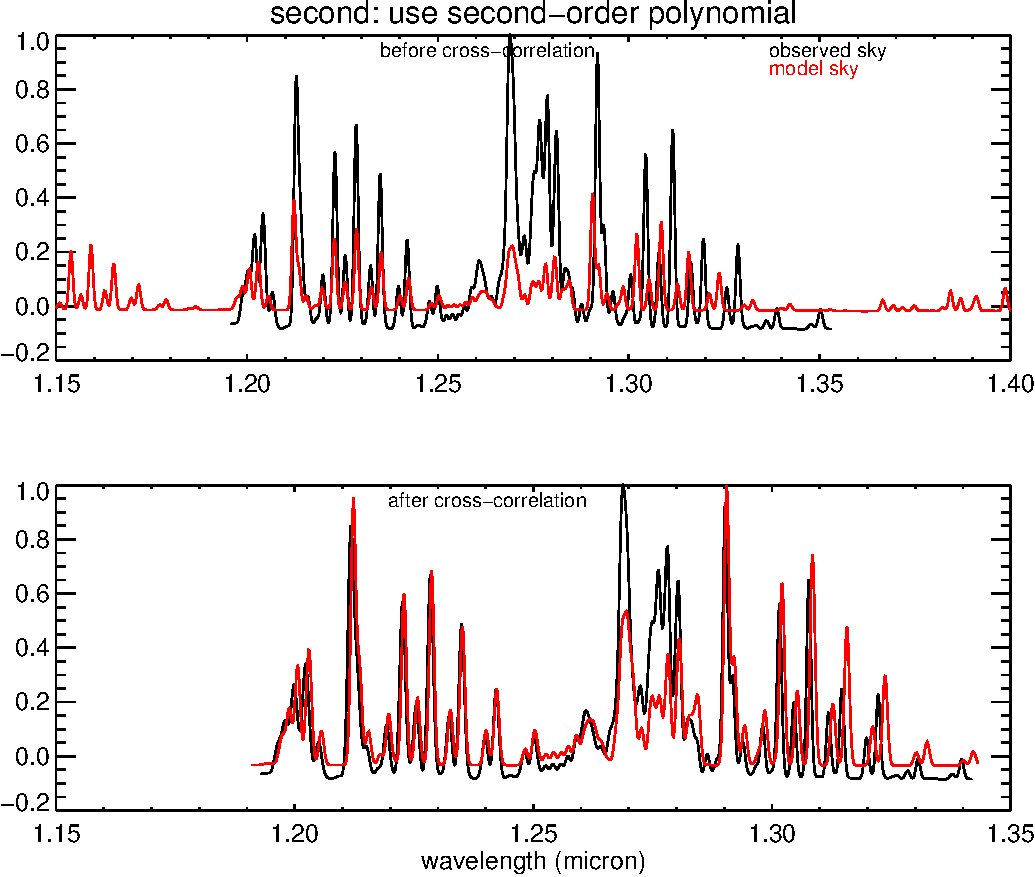
\includegraphics[width=0.31\textwidth]{wavecal2}
  \hspace*{0.01\textwidth}
 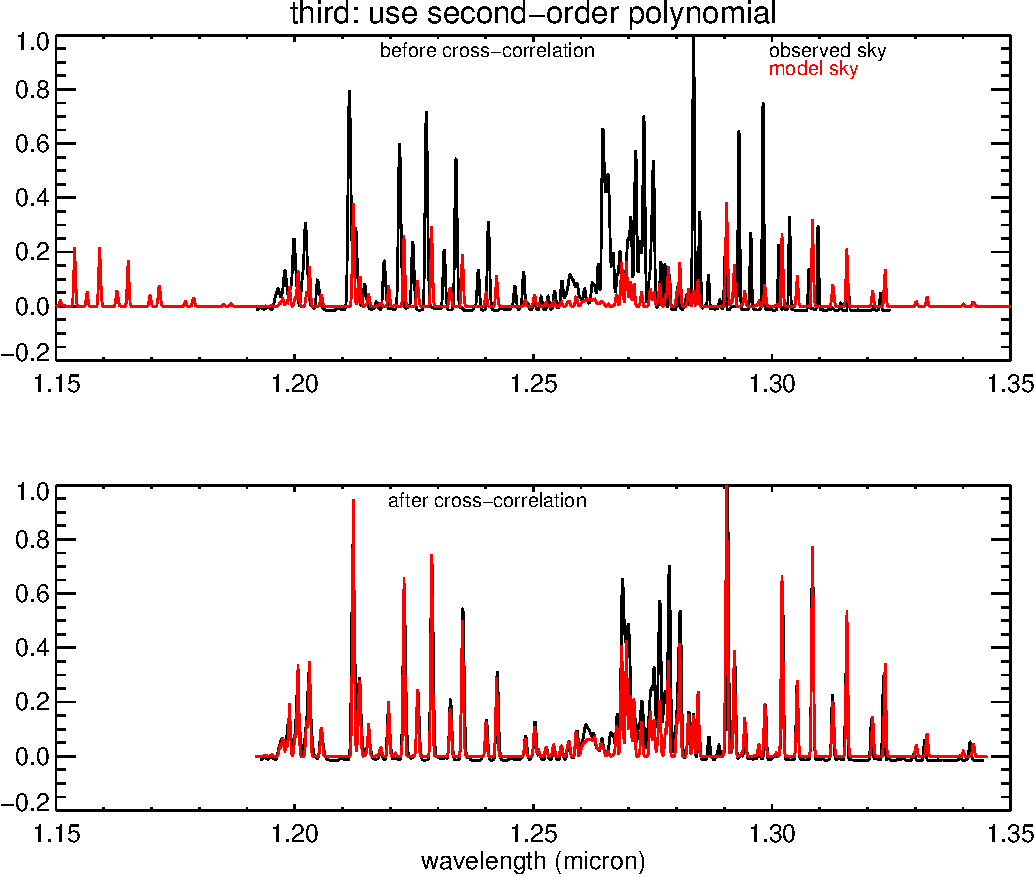
\includegraphics[width=0.31\textwidth]{wavecal3}
\end{minipage}
\caption{Approximate wavelength calibration. The sky spectrum (in black) is extracted from the central region of the slit, and is compared to a template spectrum (in red). The top panels show the initial guess, and the bottom panels show the results of the cross-correlation. The cross-correlation is repeated three times using successively higher spectral resolution.}
\label{fig:wavecal_approx}
\end{figure*}


% ---------------------------------------------------
\subsection{\texttt{flame\_findlines}}
\label{sec:findlines}


The previous procedure gives only a rough wavelength calibration that is valid for the pixel rows at the center of the slits. Since the wavelength solution typically varies with spatial coordinate within the slit (particularly for tilted slits), the calibration needs to be calculated for each individual pixel row, which is done in this step.

Initially, the spectrum of the central pixel row is extracted, and the individual OH emission lines are identified using the rough wavelength solution. A Gaussian fit is performed on each line, and the $x$ pixel coordinate corresponding to the center is stored. It is therefore necessary that the calibration found in the previous step is accurate to within the window used in the Gaussian fit, otherwise the identification of the OH lines will not be possible. The relation between the $x$ coordinate and the expected wavelength of each OH line is then fit with a low order polynomial (see example in Figure \ref{fig:speclines}). This procedure is then repeated for the next pixel row, using the wavelength solution from the previous pixel row as first guess. This is always a good assumption as long as the wavelength solution varies smoothly with position, without abrupt changes from one pixel position to the next. After all the pixel rows have been processed, the final result is a number of $x,y$ coordinates of detected OH lines, which is stored in the \fuel\ structure.

\medskip
\noindent
\textbf{Outputs.} In the slit directories, the file \code{summary\_line\_identification.ps} should be checked to get an idea of the quality and quantity of line identification. From these plots it is possible to see if there are frames with a low number of line identification, if the lines cover the 2D spectra uniformly, and what is the frame-to-frame drift along the spectral direction. A corresponding text file lists the wavelength of all the lines that were identified so that problematic lines can be easily identified and, if needed, removed from the line list. For a more thorough examination of individual frames, the \code{*speclines.ps} files show the identifications and the temporary wavelength solution for each individual pixel row in each frame. The \code{*speclines.reg} files can be loaded in ds9 on top of the corresponding cutout to see the individual detections, as shown in Figure \ref{fig:speclines}. Line identification are shown at each pixel row with red crosses; blue crosses mark those lines for which the wavelength is not accurately known, and that will be used for the rectification but not for the absolute wavelength calibration.

When using arcs, the summary files is not generated, but the \code{*speclines.ps} file for the arcs should be checked instead.

\medskip
\noindent
\textbf{Troubleshooting.} The first thing to check in case of poor line identification is that the previous step was successful. Without a reasonable starting guess for the wavelength solution it will not be possible to correctly identify and measure the lines. If the lines are far apart and there is no risk of mis-identifying them, it is possible to widen the window around the expected wavelength used to search for the line. This helps particularly if the quality of the rough wavelength calibration is poor.

In cases where the lines are very weak or infrequent (for example in some spectral regions in the K band), it may be necessary to tweak the settings in order to change the minimum number of lines identified on a single pixel row required to fit a wavelength solution, or the polynomial degree of the solution itself. It is also possible to stack multiple contiguous rows before attempting the line identification. This can be helpful when the lines are faint and a single pixel row does not have enough signal for a Gaussian fit.


\begin{figure}[tbp]
\centering
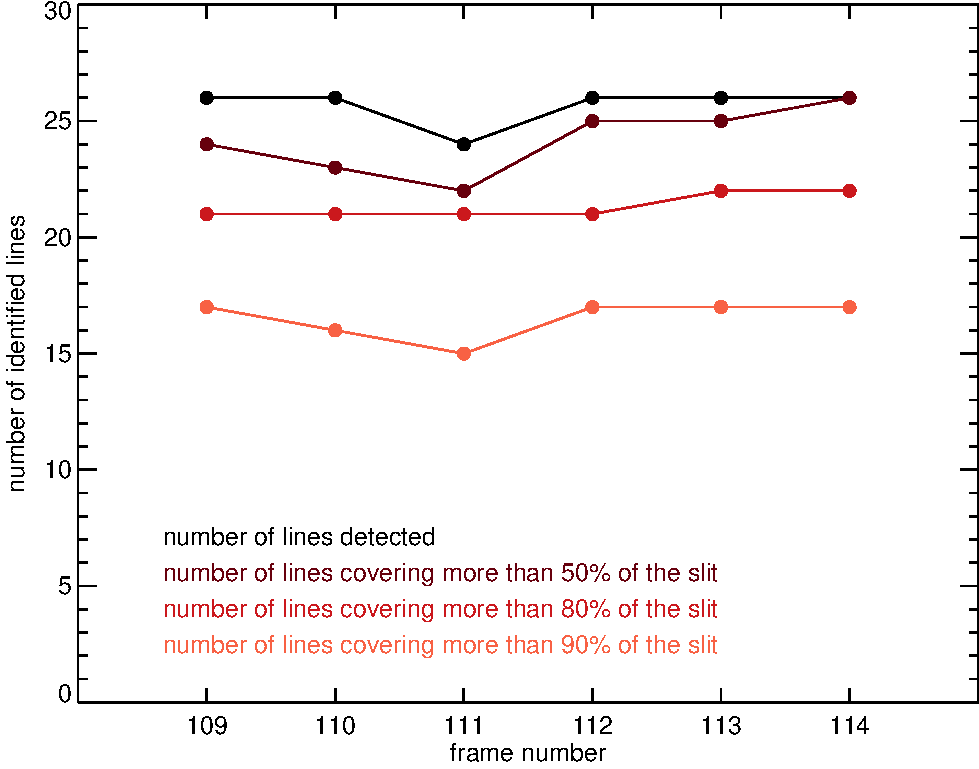
\includegraphics[width=0.7\textwidth]{number_lines}
\caption{Number of sky lines that were identified and fit with a Gaussian, as a function of frame number. The different colors correspond to different definition of ``identified lines''. The black line correspond to the total number of sky lines that were detected in at least one pixel row; the other lines show increasingly stricter definitions.}
\label{fig:number_lines}
\end{figure}


\begin{figure}[tbp]
\centering
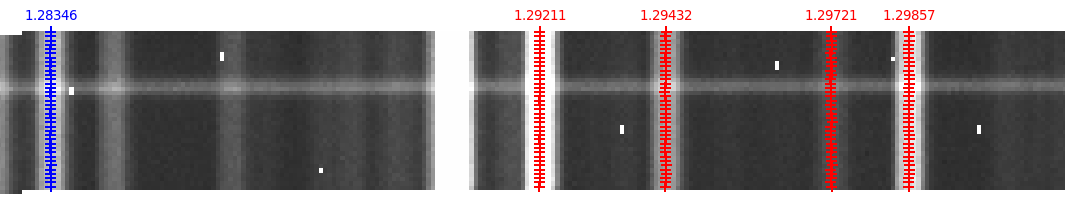
\includegraphics[width=\textwidth]{speclines.png}
\caption{Identification of sky lines. At each pixel row and for each sky line a red cross mark the peak of the Gaussian fit. Lines shown in blue lack a precise wavelength measurement, and will be used only to constrain the rectification.}
\label{fig:speclines}
\end{figure}


% ---------------------------------------------------
\subsection{\texttt{flame\_wavecal}}
\label{sec:wavecal}

For each cutout, the complete set of line identifications is used to find the best-fit wavelength solution. This is a 2D polynomial function that describes the coordinate transformation $\lambda(x,y)$. The coefficients describing this transformation are saved in the \fuel\ structure.

\medskip
\noindent
\textbf{Outputs.} In the slit directories, the files \code{summary\_wavecal.ps} and  \code{summary\_wavecal.txt} give an overview of the wavelength calibration for all cutouts. The text file and the first plot in the ps file show the residuals as a function of wavelength. This is useful for two reasons: 1) lines that are clearly off the wavelength solution can be easily identified and removed from the line list; 2) if the residuals show a systematic trend with wavelength, a higher polynomial degree may be needed for an accurate wavelength solution. The second plot shows the line widths as a function of frame number, to test that the spectral resolution is constant throughout the observations. The third plot (see Figure \ref{fig:residuals}) shows the wavelength residuals as a function of frame number. At each frame, the median and the central 68\% levels are shown in red, while the blue bars mark the median absolute deviation.

For each slit and cutout, the \code{*wavecal.ps} files show a map of the line identifications, a plot of the measured line widths, and one of the wavelength residuals. In all these plots, the line identifications that have been discarded during the fit of the wavelength solution are marked in red. When using arcs, the \code{*wavecal.ps} files show the fit to the sky lines from which the wavelength shift is calculated.

When using arcs, the summary files is not generated, but the \code{*wavecal.ps} file for the arcs should be checked instead.

\begin{figure}[tbp]
\centering
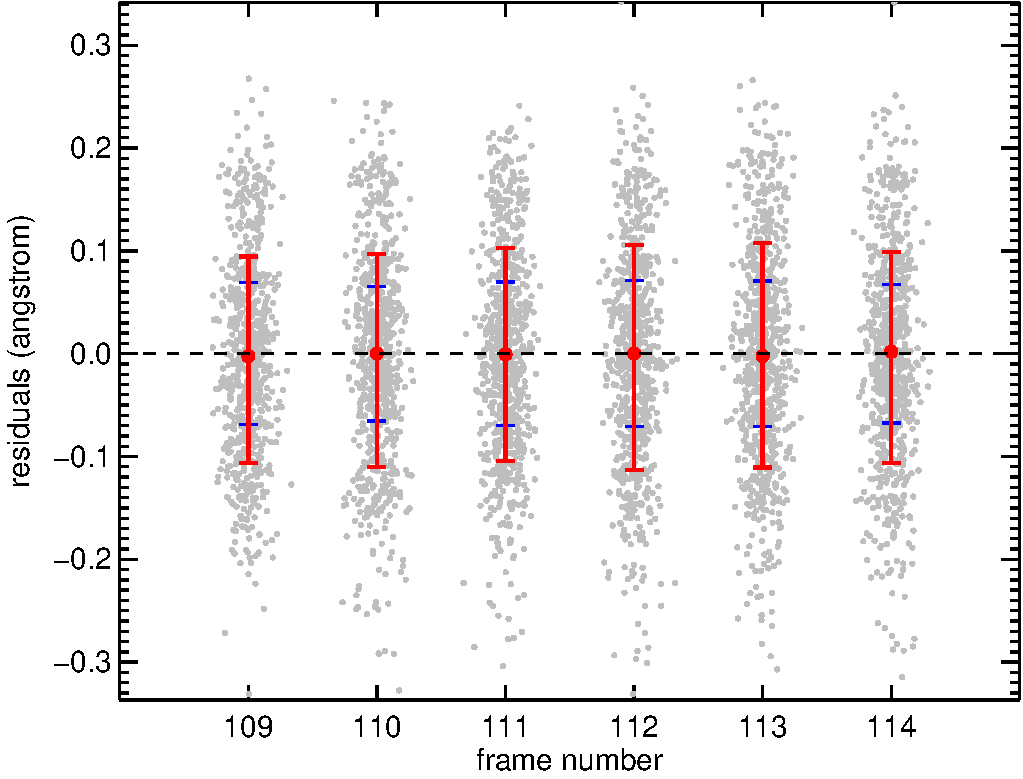
\includegraphics[width=0.7\textwidth]{residuals}
\caption{Residuals of the wavelength calibration. For each frame, at each pixel row each sky line is fit with the Gaussian and its position is measured. Then its wavelength is calculated using the best-fit 2D wavelength solution. The difference between this value and the true wavelength of the sky line is then shown here as a gray point. For each frame the median and 68\% levels are shown in red. The MAD (median absolute deviation) is a better estimate of the level of wavelength precision that can be expected, and is shown in blue (in both positive and negative values; i.e. the distance between the two blue bar is twice the measured MAD).}
\label{fig:residuals}
\end{figure}


\medskip
\noindent
\textbf{Troubleshooting.} If the residuals show strong trends with wavelength, it is possible that a higher order polynomial is needed for an appropriate description of the wavelength solution. The default orders are 3 along the $x$ axis and 2 along the $y$ axis, and can be changed using the corresponding settings. It is also possible to change the criterion for outlier rejection, which can have a strong impact on the quality of the resulting wavelength solution. By default, line measurements that are more than 3-sigma away from the 2D wavelength solution are rejected, but this can be changed via the \code{wavecal\_sigmaclip} setting.

It is possible that some of the emission lines are systematically off due to inaccuracies in their wavelengths saved in the line list. This can happen for various reasons including blended lines, especially when the spectral resolution does not match exactly that of the line list. In these cases it is best to remove by hand these lines from the line list. The file with the line list is saved in the intermediate directory, and its name is stored in \code{settings.linelist\_sky\_filename} (or \code{settings.linelist\_arcs\_filename} when using arcs). The recommended procedure is the following: make a copy of the file, edit it by removing the problematic lines, then edit the file name in \code{settings.linelist\_sky\_filename}, and run again the last two steps, i.e. from \code{flame\_findlines}.

When using arcs, the default behavior is to extract the sky spectrum anyway, identify sky lines of known wavelength, and calculate the shift in wavelength with respect to that solution derived from the arcs (and additional figures are saved in the \code{*wavecal.ps} files. This shift is calculated for each cutout and applied to the wavelength solution, even in those cases where only one sky line is present in the observed spectrum (this situation is rarely seen in the near-infrared but common in the optical). It is possible to specify a minimum number of sky lines that should be identified before applying this shift. If not enough sky lines are identified, the shift is calculated by cross-correlating the observed sky spectrum with a model. This procedure, however, is not very robust when the sky emission is faint, especially at very blue wavelengths ($\lambda < 6000\AA$). It is also possible to switch off the wavelength shift by setting \code{shift\_arcs}$=0$ (the shift is still calculated but is not applied).


% ---------------------------------------------------
\subsection{\texttt{flame\_illumcorr}}
\label{sec:illumcorr}

The illumination correction is calculated from the sky lines, the arcs, or the illumination flat, and is applied to each cutout. The user can choose to skip this step by setting the parameter \code{illumination\_correction}$=0$.

\medskip
\noindent
\textbf{Outputs.} For each cutout, the corresponding illumination-corrected FITS file (\code{*illcorr*.fits}) is created. From now on, this is the file that will be used in the data reduction. A figure is also saved in the \code{*illumcorr.ps} files, showing the measured flux across the slit in black, and the smooth model in red.



% ---------------------------------------------------
\subsection{\texttt{flame\_skysub}}
\label{sec:skysub}

Because the OH emission lines vary on short timescales, the A-B subtraction typically leaves strong residuals. In order to improve the sky subtraction, \flame\ constructs and subtracts a model of the sky, following the method of Kelson 2003. \flame\ performs this operation on each frame for every slit, and saves a FITS file of the sky-subtracted data.

This step improves substantially the quality of the data reduction, however it can be demanding from the computing point of view, particularly for very tall slits. If the user wants to skip this step to obtain a quick reduction, it is sufficient to set \code{skysub=0}. Also, if the target is extended and covers most of the slit, an accurate model of the sky cannot be constructed, and this step may well be skipped altogether.

It is possible, by setting \code{skysub\_plot=1}, to have a pop-up window showing the sky emission spectrum (collapsed onto one dimension) and the B-spline fit for every frame. This can be a useful diagnostic to check the quality of the sky model. It is usually preferable to have the plot zoomed in on a region rich of sky lines; the region can be set via the keyword \code{skysub\_plot\_range}. By default this pop-up window is not activate because in some machines it can significantly slow down the data reduction.


\medskip
\noindent
\textbf{Outputs.} IN each slit directory, the \code{*skymodel.fits} files contain a 2D model of the sky emission for each cutout. These models are subtracted from the observed frames and the results are stored in the \code{*skysub.fits} files.


\medskip
\noindent
\textbf{Troubleshooting.} The most common problem with the sky subtraction is a wavy shape of the sky line residuals in the sky-subtracted frames. However, when this happens the problem does not lie in the sky subtraction itself, but in the inadequate wavelength solution. Users in this case should go back to the wavelength calibration step or even the line identification step and understand what went wrong.

Another common problem is the over-subtraction due to bright emission (either line or continuum) from the target. In order to avoid subtracting the target itself, at each wavelength a generous outlier rejection is performed before fitting the sky model. Here is how the rejection works: within a given wavelength window, pixels are ranked by brightness; a fixed fraction of pixels with the most extreme values are rejected; then this procedure is repeated. For bright or extended targets this rejection should be more aggressive. This can be obtained by increasing the rejection fraction and/or the number of loops. Note that the total number of rejected pixels is uniquely determined (within rounding effects due to the relatively small number of pixels) by these two quantity. For example, the default values are 3 loops in which 10\% of pixels are rejected, therefore $(1-0.10)^3=0.729$ is the remaining fraction, corresponding to a total rejection fraction of 27\%. The window used for the rejection can also be tweaked to the typical wavelength over which the target and/or the sky spectrum vary.

One important parameter for modeling the sky is the positioning of the breakpoints of the B-spline function. By default, the distance between breakpoints is equal to the size, in wavelength units, of a pixel. However this may not be the optimal choice: when the slit is tall and the sky lines are slightly tilted, the sampling of the sky spectrum is much higher - easily by a factor of 10 or more - then the size of an individual pixel. \flame\ takes advantage of this to obtain a very accurate description of the sky spectrum; see Kelson (2003) for details. In these cases the default choice of breakpoints may be too coarse, with a consequent poor sky subtraction. Figure \ref{fig:bspline} shows an example of this, where the default choice (central panel) leads to a "striped" pattern at the position of the sky lines in the sky-subtracted frame. Users can change the sampling with the setting \code{skysub\_bspline\_oversample}, which defines the distance between successive breakpoints in units of spectral pixels. The default value is 1 and can be changed to any integer or inverse of integer (...1/3, 1/2, 1, 2, 3...).


\begin{figure}[tbp]
\centering
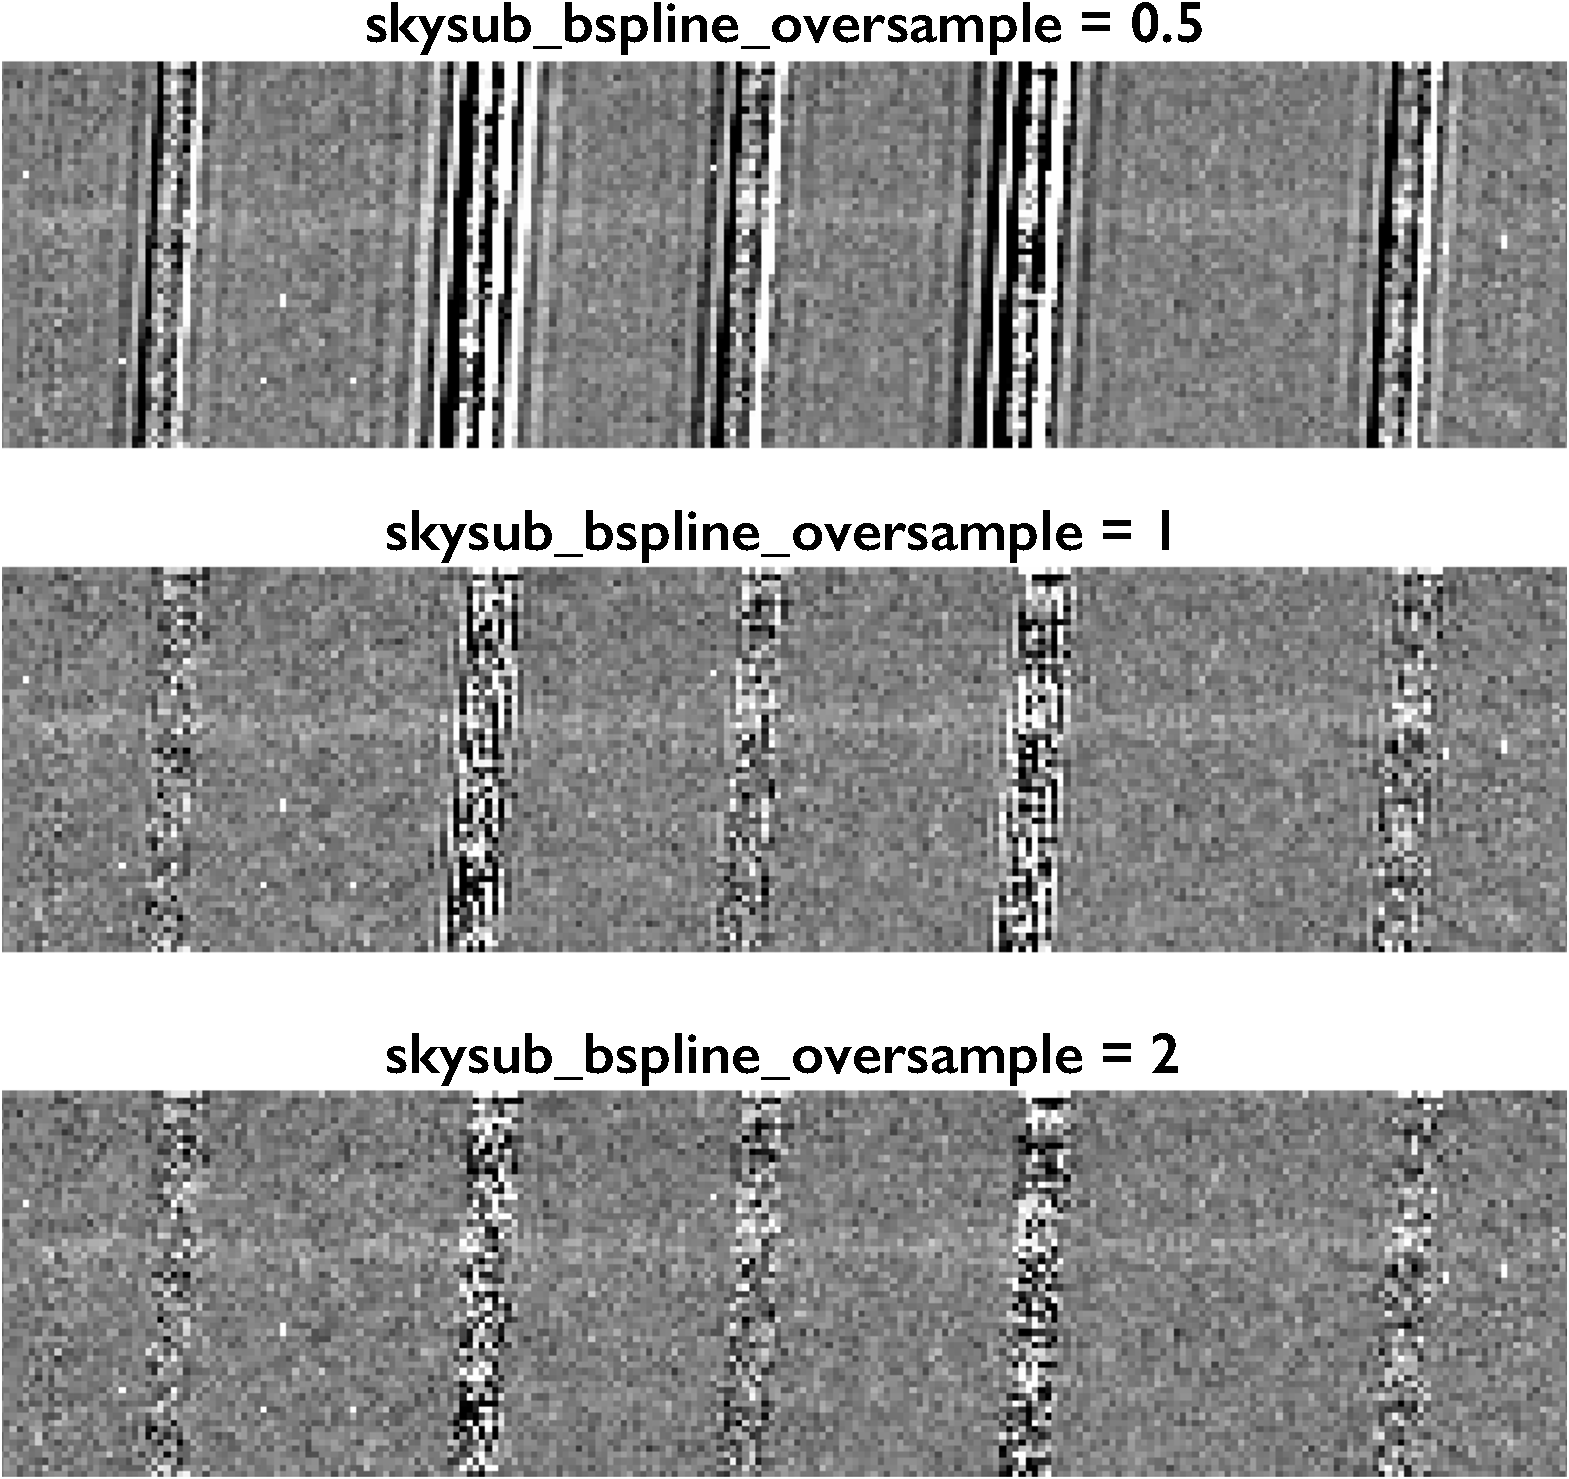
\includegraphics[width=0.5\textwidth]{oversample}
\caption{Effect of changing the distance between B-spline breakpoints on the sky subtraction. From top to bottom, this distance is set to half, one, and two times the size of spectral pixels. Since the slit is relatively tall and the wavelength solution is slightly tilted, a large number of breakpoints is required for an optimal sky subtraction.}
\label{fig:bspline}
\end{figure}


% ---------------------------------------------------
\subsection{\texttt{flame\_rectify}}
\label{sec:rectify}

Using the 2D rectification coefficients calculated in \texttt{flame\_wavecal\_accurate}, this step performs both the wavelength calibration and the spatial rectification simultaneously, using only one interpolation. The interpolation is calculated using the IDL function \code{griddata}, and the interpolation method can be set via the settings to one of the following: 'NaturalNeighbor' (default), 'Linear', 'NearestNeighbor', or 'Quintic'. These methods are explained in detail in the IDL documentation.

\medskip
\noindent
\textbf{Outputs.} Each cutout is rectified and saved as a \code{*rectified.fits} file. Additionally, the sky-subtracted frames and the frames with the 2D model of the sky are also rectified and saved as FITS files.

\medskip
\noindent
\textbf{Troubleshooting.} When the slits are very tall, which happens often when dealing with longslit data, the default 'NaturalNeighbor' method can introduce artifacts in the rectified frame. In these cases the 'Linear' method tends to perform better. Setting the method to 'Linear' can also significantly speed up the data reduction.



% ---------------------------------------------------
\subsection{\texttt{flame\_combine}}
\label{sec:combine}

This step consists in the stacking of all the A and B frames. Sigma-clipping is first performed to remove cosmic rays and bad pixels, the default value is 2-sigma but this can be changed. The individual A and B stacks, and the difference A-B, are output as FITS file for each slit. Non-skysubtracted versions of the stacks are also saved.

If the dithering length, as calculated from the star traces, matches the distance between any two slits, then these are assumed to be matching slits and their A-B stacks are combined together. This assumption breaks down if the star traces for the A and B positions actually belong to different stars.

By default, no weights are applied to the frames, but the user can set frame\_weights to 'None', 'Flux', 'Seeing', or 'Peak'.

\medskip
\noindent
\textbf{Note:} From this step the outputs are saved in the \code{output} directory.

\medskip
\noindent
\textbf{Outputs.} When adopting an $A-B$ nodding, the file \code{slit\_pairing.ps} shows the positions of all slits in the A and in the B frames. From this plot it should be clear whether the nod is off-slit, on-slit, or paired slits (see Figure 2 of the paper).

The FITS file output by this step represent the main product of the pipeline, and are organized into two directories: \code{spec2d/} and \code{spec2d\_skysub/}. The two directories contain the same number of files, with identical names, but differ from whether the model sky has been subtracted from individual cutouts or not. If one is not interested at all in the sky-subtracted results and wants to increase the speed of the data reduction, the settings \code{skysub} can be set to zero, and only the \code{spec2d/} directory will be created.

Each of these directories contain a number of files. For multi-slit data, the files \code{mosaic\_SNR.fits} and \code{mosaic\_flux.fits} give an overview of the reduced data, which are combined back into a mask following the same order as the original frames. This is useful for example to count the number of detections, or to compare the spectra of different slits, etc; however these files should NOT be used for the scientific analysis.

For each slit, the science-grade reduced spectra are saved as individual FITS files. \code{slitXX*\_A.fits} is the stack of all the A frames, and is the only type of file that is always produced independently of the type of observations and nodding strategy. When nodding, then \code{slitXX*\_B.fits}, the stack of all the B frames, is also saved. Additionally, the difference of these two stacked is saved as \code{slitXX*\_A-B.fits} and \code{slitXX*\_B-A.fits}. The latter is simply the opposite of the former, and is saved only in order to streamline the following step. For on-slit nodding, these frames contain the flux of the target split into a negative and a positive trace. Therefore the last step is to add the $A-B$ to the shifted $B-A$ in order to make the final spectrum. This is saved as \code{slitXX+slitXX.fits}, and shows the characteristic negative-positive-negative pattern of on-slit observations. Note that the flux is entirely contained in the positive trace; the two negative traces do not contain additional data as their sum is identical to the positive trace. If, instead, the slits are paired during the observations, so that the target falls in slitXX during the A frame and in slitYY in the B frame, then the final output will be \code{slitXX+slitYY.fits}, and will contain only one positive trace.

Each of the science-grade spectra is a FITS file with six extensions, that can be read for example in IDL using \code{mrdfits}, and can be visualized calling ds9 with the option \code{-multiframe}. This is the content of the extensions:
\begin{enumerate}
\item flux (in electrons per second)
\item theoretical error (in electrons per second)
\item empirical error (in electrons per second)
\item model of sky flux (in electrons per second)
\item map of exposure time (in seconds)
\item weight map (with the default settings this corresponds to the number of frames that were combined, at each pixel position)
\end{enumerate}


\begin{figure}[tbp]
\centering
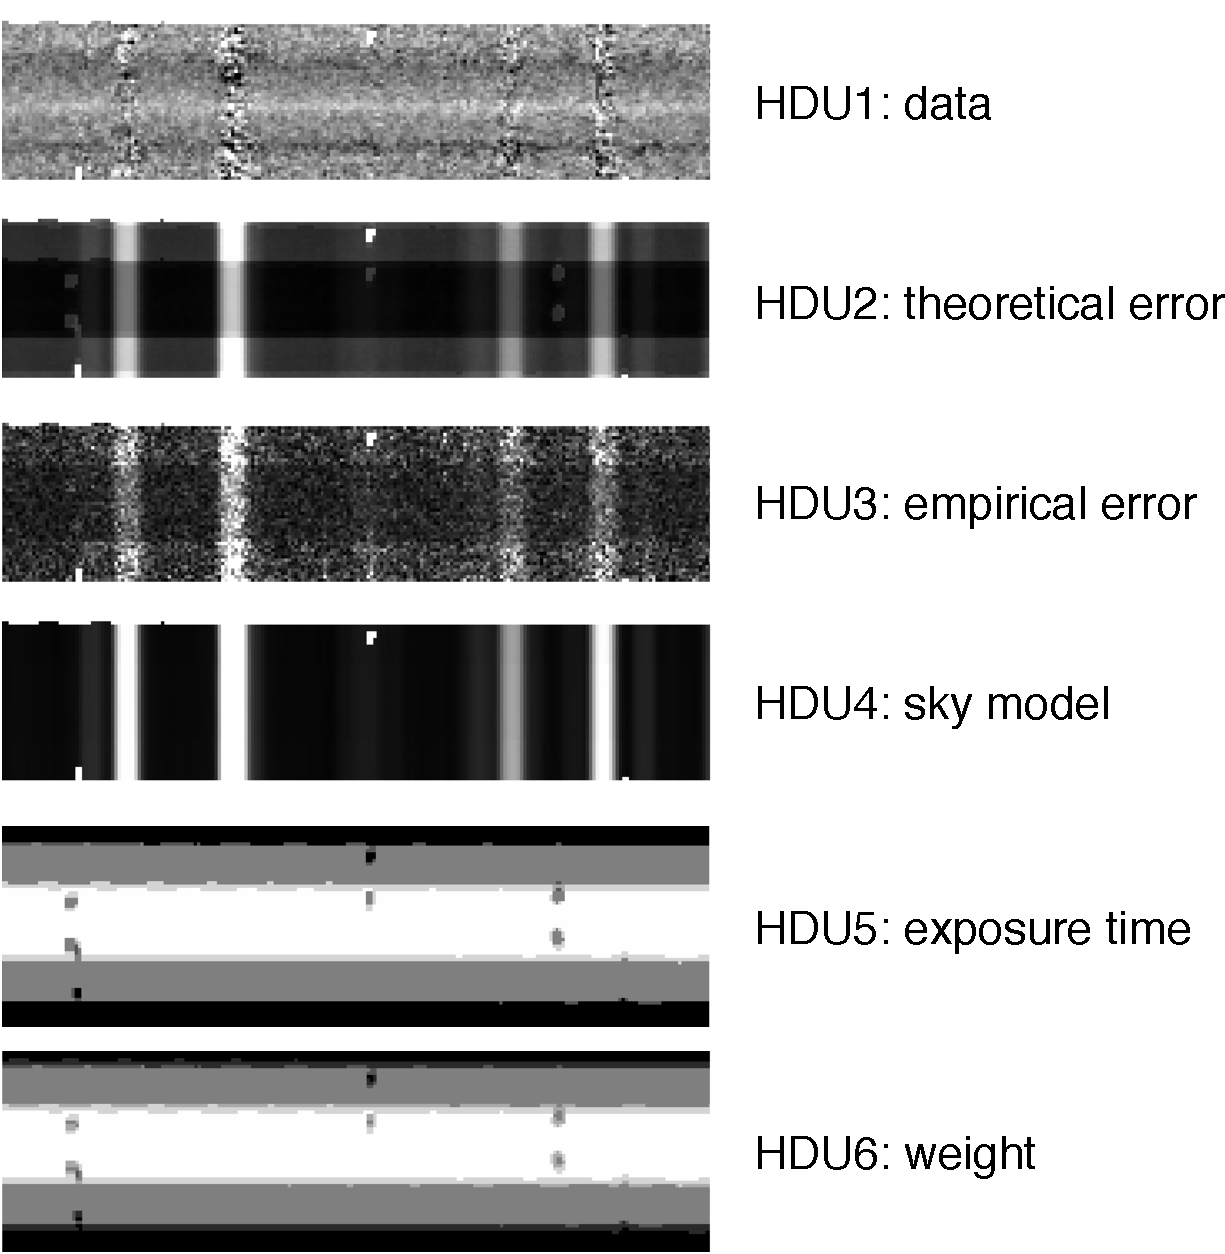
\includegraphics[width=0.6\textwidth]{extensions}
\caption{Each science-grade 2D spectrum contains six extensions, or HDUs. In this example, a small portion of the spectrum is shown for a LUCI observation obtained with on-slit nodding, as shown by the negative-positive-negative pattern in the first extension.}
\label{fig:extensions}
\end{figure}



% ---------------------------------------------------
\subsection{\texttt{flame\_checkdata}}
\label{sec:checkdata}

This module performs a quality check on the reduced data set. Its only purpose is to produce diagnostic plots, saved in the output directory, that can be used to judge the quality of the observations and of the data reduction.

\medskip
\noindent
\textbf{Outputs.} If present, the reference star spectrum is analyzed and the effective seeing calculated. The file \code{reference\_star.ps} is written, showing the spatial profile, the width and position of the stellar track as a function of wavelength, and the extracted 1D spectrum of the star.

For each slit, a \code{*.ps} file containing a number of plots is saved. The first plot shows the stacked sky spectrum, from which the sky lines are identified and fit, and the wavelength residuals and spectral resolution R are shown. Stats on the wavelength solution and the velocity resolution are shown at the bottom. The remaining plots are identical to those produced by the \texttt{flame\_wavecal} step, and illustrate the performance of the wavelength calibration.

These diagnostics are based on the measurement of sky emission lines. When arcs are used instead, the files show the result of a comparison between the sky spectrum and a template, with the purpose of checking the accuracy of the arcs-based wavelength calibration.



% ---------------------------------------------------
\subsection{\texttt{flame\_extract}}
\label{sec:extract}

This is the last module, which identifies the brightest object in each slit and extracts the 1D spectrum. Optimal extraction is used, but setting \code{extract\_optimal=0} forces boxcar extraction. When using optimal extraction, the weights are determined by fitting a Gaussian function to the observed profile (i.e., the 2D spectrum collapsed along the wavelength direction). However, for bright targets it may be better to derive the weights directly from the observed profile; this can be achieved setting \code{extract\_gaussian\_profile=0}.

\medskip
\noindent
\textbf{Outputs.} Similarly to what done for the 2D spectra, the extracted spectra are saved into two directories: \code{spec1d/} and \code{spec1d\_skysub/}, respectively without and with model-based sky-subtraction (but the $A-B$ subtraction is always applied, if possible). These directories include, for each slit, a ps file showing the spatial profile with its Gaussian fit, the extracted spectrum, and the SNR for both the boxcar extraction and the optimal extraction; and a FITS file containing the extracted spectrum. This is stored as a structure containing the fields \code{lambda} (wavelength in units of angstrom), \code{flux} (in electron per second), \code{ivar} (inverse variance), \code{ivar\_emprical} (inverse variance calculated from the empirical error spectrum), and \code{sky} (sky spectrum extracted from the 2D model). The error spectrum can be easily obtained as $\mathrm{err} = 1/\sqrt{\mathrm{ivar}}$. Note that the FITS file is not produced if the automatic identification of the target in the 2D spectrum fails, which can happen if the emission is faint or concentrated in a few emission lines, or if the slit is very tall and the trace of the target is lost in the noise or in the large-scale detector systematics.

There are a number of third-party programs that can be used to visualize and analyze the extracted 1D spectra. In particular, the FITS files output by \flame\ are compatible with the interactive programs SpecPro and SpecViz.

SpecPro\footnote{\url{http://specpro.caltech.edu/}} is written in IDL. It uses both the IDL Astronomy User's Library and the mpfit routines, which are also required by \flame. After downloading and installing the source code, simply launch IDL from the \code{extraction/} directory and run the \code{specpro} command.

SpecViz\footnote{\url{https://github.com/spacetelescope/specviz}} is written in Python. After installing SpecViz, copy the configuration file \code{flame/external/flame.yaml} to the \code{\textasciitilde/.specviz/} directory. This file contains a description of the data format used by \flame. Open SpecViz, click the \emph{Open} button, and in the dropdown menu \emph{Files of type} there should now be an entry called \emph{Flame data reduction pipeline}. Note that it is not necessary to select the file type every time you open a spectrum; SpecViz should be able to automatically recognize the file and correctly read in the \flame\ output.


% ---------------------------------------------------
\subsection{Directory structure and final output}
\label{sec:final_output}

Explain that you can delete the intermediate directory.


% ---------------------------------------------------
\subsection{Combining different data sets}

Commonly, observations of the same target are split over many nights or even runs. In these cases it is best to reduce individual chunks independently and then combine the resulting 2D spectra. This can be done using a provided IDL procedure \code{flame\_util\_combine\_spectra}. The IDL file has a detailed description of its usage and of the options available. For example, to combine three fully reduced 2D spectra of the same target obtained over three different nights, one would run
\begin{lstlisting}
  flame_util_combine_spectra, ['slit07_night1.fits', $
    'slit07_night2.fits', 'slit07_night3.fits'], $
    /rectified_frame, /NaN, /usesigma
\end{lstlisting}
The output 2D spectrum has the same format as those output by \flame.

Different options exist for the weights to be used when combining the data (in the example above, the sigma image is used in order to optimize the SNR) and for the type of spatial alignment. In most cases the alignment should be done on the rectified frame, assuming that the same reference star was used for all observations. However sometimes this is not possible, for example when no reference star was observed. If a spectral features such as an emission line is detected in each individual spectrum, this can be used to align the frames, by providing the pixel coordinates for an 'alignment box' in which the spectral feature is located.

The utility \code{flame\_util\_combine\_spectra} can also be used to combine parallel observations of the same target obtained with LUCI1 and LUCI2. Note that for some configurations the two instruments have a slightly different spatial scale. Spatial resampling is needed before the data from the two eyes can be properly combined. This resampling should be done during the data reduction, as explained in Section \ref{sec:spatialcal}.

Finally, a simple boxcar extraction can be performed manually on a 2D spectrum like this:
\begin{lstlisting}
  flame_util_extract_spectrum, 'slit07.fits', $
    yrange=[52,58]
\end{lstlisting}
where \code{yrange} is an integer array specifying the first and last pixel rows (in detector coordinates) to be considered for the extraction. The 1D spectrum is then saved as a FITS file in the same format as for the files output by \code{flame\_extract}.




% ***********************************************************************************************
% ***********************************************************************************************
%									5. OTHER INSTRUMENTS
% ***********************************************************************************************
% ***********************************************************************************************

\section{Supported Instruments}
\label{sec:instruments}

All the \flame\ modules described in Section \ref{sec:data_reduction} are written in an instrument-independent way, and can be used on nearly any optical or near-infrared data set. The instrument-specific part is relegated to the initialization module. When running \flame, the correct initialization module must be called, and those options that are required and/or relevant to the specific instrument must be set. To simplify this procedure, a different driver file is available for each instrument, although in principle a skilled user should be able to easily write the correct driver for any supported instrument. All driver files are split into three parts:
\begin{enumerate}
  \item The inputs are set, in slightly different ways for different instruments.
  \item The specific initialization module is then run and the \fuel\ structure is created.
  \item The data reduction modules are called. This part is identical for all drivers.
\end{enumerate}

The list of files in the \texttt{flame/drivers/} directory shows what instruments are supported. Currently, this directory contains the following files:
\begin{itemize}
  \item[] \texttt{flame\_driver\_luci.pro}: driver for reducing data from the LUCI1 and LUCI2 instruments at the Large Binocular Telescope.
  \item[] \texttt{flame\_driver\_mosfire.pro}: driver for reducing data from the MOSFIRE near-infrared instrument at the Keck telescope.
  \item[] \texttt{flame\_driver\_lris.pro}: driver for reducing data from the blue and red channel of LRIS at the Keck telescope.
  \item[] \texttt{flame\_driver\_minimal.pro}: minimalistic driver that can be used to run the first two modules (diagnostics and quick stack) on any data set, including instruments that are not supported.
\end{itemize}

In the remainder of this section, we quickly describe each supported instrument and give indications on how to implement support for new instruments.


\subsection{LUCI at LBT}

The reduction of LUCI data is described throughout Section \ref{sec:setup} and \ref{sec:data_reduction}, and no further discussion for this instrument is needed.


\subsection{MOSFIRE at Keck}

MOSFIRE is a multi-slit near-infrared spectrograph, and its data are in many aspects similar to LUCI data, partly because both instruments use exactly the same type of detector. The data from MOSFIRE are usually simpler to reduce because the slit tilt is fixed, and has been chosen to optimize the spectral sampling of the sky lines. The angle of the dispersive element is also fixed, so that for a given band (Y, J, H or K), the observed wavelength range depends exclusively on the spatial placement of the slit.

The header of MOSFIRE data contains very detailed information on the slitmask configuration, and usually the slit identification presents no issues. Given the excellent spatial sampling of the sky spectrum, a higher value of the bspline oversampling is generally needed (although this is automatically set to a high value during the initialization).

Note that MOSFIRE has an official data reduction pipeline\footnote{\url{http://keck-datareductionpipelines.github.io/MosfireDRP/}} which is excellent, although less flexible than \flame.


\subsection{LRIS at Keck}

LRIS is an optical multi-object spectrograph at Keck equipped with a blue and a red arm. The initialization module included with the Flame distribution will change the settings according to which arm has been used.

Data reduction for the red arm is not very different from what described above for near-infrared data: the data are dominated by sky lines, that can be used to derive the wavelength calibration. Usually A-B nodding is not performed, because the model sky subtraction is sufficient given that the sky emission is not as strong as in the near-infrared.

Data taken with the blue arm look significantly different given the almost complete absence of sky emission lines, and the presence of a very faint sky continuum. This means that the sky subtraction is not very problematic, and nodding is almost never necessary. However, the lack of sky lines introduces an additional difficulty: the wavelength calibration cannot be obtained directly from the data, and has to be derived using dedicated observations of lamp arcs. These calibrations should be taken as close as possible to the science data in terms of time and elevation, to avoid spectral and spatial shifts (see Section \ref{sec:wavecal} for details).

Given the weaker sky emission, individual frames taken in the optical have generally longer exposure times compared to near-infrared observations. This means that cosmic rays can be very numerous (especially in the red arm), and there may not be sufficient frames for an effective sigma-clipping. In these cases it is recommended to apply L.A.Cosmic to individual frames to mask out bad pixels and cosmic rays.


\subsection{Diagnostics for unsupported instruments}
\label{sec:minimal}

The diagnostics plots produced by \flame\ are particularly useful for monitoring the conditions (seeing, transmission, and drift) while observing. In order to make these products available to the wider community of users, \flame\ contains an initialization module that can be used with almost any type of spectroscopic data. This "minimal" module has basic assumptions on the data format: each frame must be a FITS file with a single HDU, and the wavelength runs along the horizontal direction. The only parameter required is the spatial pixel scale of the instrument. The associated driver file \texttt{flame\_driver\_minimal.pro} performs only the first two steps of the data reduction, producing the diagnostics plots and the quick stack. In order to proceed further, a fully functional initialization module is needed.

\subsection{How to add support for a new instrument}

In order to use \flame\ with an instrumnt beyond those officially supported, it is necessary to write an initialization module. This can be built easily starting with the provided template \texttt{flame\_initialize\_template.pro}. The initialization module takes the \inp\ structure and as its only argument, and outputs a complete \fuel\ structure. The first step is always to create a default \fuel\ structure using the provided utility function. Then the initialization module must perform the following operations.

\subsubsection{Information on the instrument}

The appropriate \code{fuel.instrument} structure, containing a set of parameters such as the spectral resolution, spatial pixel scale, etc, must be created. The required parameters are listed in Table \ref{tab:instrument}. Nearly all instruments have one or more parameters that can be changed; in these cases it is important that the \code{instrument} structure contains the values that are correct for the specific data set. Typically these parameters can be derived from the FITS header of the first science frame. Note that the instrument structure can include any number of extra parameters that are not listed in the Table, such as the instrument name, the filters, the configuration of the dispersing element, etc. This is encouraged for two reasons: first, it makes it easier to write a clean initialization module, where the instrument structure is passed to different function to calculate additional quantities (see following points); secondly, it constitutes important archival information that can be easily read from the \fuel\ structure, which is always saved together with the main output of the pipeline.


 % ******************************************************************************
 \begin{table}
 \caption{Required fields of the \code{fuel.instrument} structure \label{tab:instrument}}
 \medskip
 \footnotesize
 \makebox[\textwidth][c]{
   \begin{tabular}{ll}
     \hline
     \smallskip
     Field    & Description \\
     \hline
     \smallskip
pixel\_scale                & spatial pixel scale, in arcsec per pixel \\
resolution\_slit1arcsec     & approximate spectral resolution R for a slit width of 1 arcsec \\
gain                        & detector gain, in units of electrons per ADU \\
readnoise                   & detector readnoise, in units of electrons \\
linearity\_correction       & array with the polynomial coefficients describing the linearity correction \\
default\_badpixel           & string with the name of the FITS file with the default bad pixel mask (can be 'none') \\
default\_dark               & string with the name of the FITS file with the default dark (can be 'none') \\
%%% CHECK THESE! \\
trim\_edges                 & (optional) integer indicating how many pixels must be discarded from each side of the detector \\
 \hline
 \end{tabular}
 }
 \end{table}
 % ******************************************************************************



\subsubsection{Information on the slits}

The \code{fuel.slits} structure, containing information on each of the slits such as the target IDs, the approximate spatial location of the slit, and the approximate wavelength range, must be created. For longslit data, this is only one structure; for multi-slit data, \code{fuel.slits} is actually an array of structures with identical fields. The required fields are listed in Table \ref{tab:slits}.


  % ******************************************************************************
  \begin{table}
  \caption{Required fields of each \code{fuel.slits} structure \label{tab:slits}}
  \medskip
  \footnotesize
  \makebox[\textwidth][c]{
    \begin{tabular}{lll}
      \hline
      \smallskip
      Field  & Example    & Description \\
      \hline
      \smallskip
 number                & 1              & unique integer number identifying the slit \\
 name                  & 'galaxy-4385'  & string with target name (does not have to be unique) \\
 skip                  & 0              & should always be zero; it can be later changed to one to skip this slit \\
 PA                    & 0.0            & position angle (in deg, can be NaN) \\
 approx\_bottom        & 680            & approximate $y$ pixel coordinate for the bottom of the slit (e.g., )  \\
 approx\_top           & 740            & approximate $y$ pixel coordinate for the top of the slit  \\
 approx\_target        & 710            & approximate $y$ pixel coordinate for the target in this slit \\
 width\_arcsec         & 0.75           & slit width in arcsec (can be NaN)  \\
 approx\_R             & 2500           & approximate spectral resolution R of this slit \\
 range\_lambda0        & [1.15, 1.25]     & allowed range for the wavelength of the first pixel (in micron) \\
 range\_delta\_lambda  & [0.0001, 0.0003] & allowed range for the wavelength scale (in micron per pixel) \\
  \hline
  \end{tabular}
  }
  \end{table}
  % ******************************************************************************


\subsubsection{Set up the line lists}

The initialization module must also select the appropriate line list (for sky and/or arcs) and make local copies in the \code{intermediate} directory. The \code{data/} directory in the \flame\ distribution contains three sky line lists for low, medium, and high spectral resolutions (respectively $R\sim$1000, 3000, and 6000), covering from the optical to the $K$ band.


\subsubsection{Edit the settings}

Finally, the default values of \code{fuel.settings} can be edited, in order to optimize the data reduction for the specific instrument. Typically, only a minority of the settings (listed in Table \ref{tab:settings}) are changed during the initialization. Examples include the type of wavelength calibration (using sky lines or arcs), the order of the wavelength solution, the spectral resolutions used during the rough calibrations, etc. Note that the user can then modify each of the settings, including those already changed by the initialization module.







\end{sloppypar}



\end{document}
